\chapter{Benchmarking QUBO solvers}\label{benchmark}
This chapter first introduces related benchmarking work that has been done for QUBO problems and QUBO solvers. Then, we present our results for the solvers and datasets used for this study.

\section{Related benchmarking work}
One of the first benchmarking works for quantum annealing was conducted by Denchev et al. \yrcite{denchev2016computational}, who measured the performance of D-Wave quantum annealing on the older D-Wave 2X machine using specially crafted problems that have tall and narrow energy barriers separating local minima. Quantum annealing is expected to be $1.8 \times 10^8$ times faster compared to simulated annealing, which tends to fail with problems with such an energy landscape.


\outcite{b34} evaluated the performance of QAOA on the IBMQ backend and the D-Wave solver using instances of MaxCut and 2-satisfiability problems with up to 18 variables. The performance of the QAOA algorithm is inconsistent and underperforms quantum annealing in their problem set. More recently, \outcite{b35} also compared the performance of QAOA on the IBMQ backend and D-Wave quantum annealing on randomly generated Ising problems with cubic interaction terms and also found that quantum annealing had superior performance over QAOA for all problem sizes.

\outcite{gomes2019classical} showed that the NNQS solving method with an RBM architecture produces good solutions for the max-cut problem with graph sizes of up to 256. \outcite{khandoker2023supplementing} uses recurrent neural networks as the NNQS architecture for the max-cut and traveling salesman problem and found that it outperforms SA. However, there is no direct study that compares performance across quantum annealing, QAOA, and NNQS.

\section{Results and Discussion}
Performance is shown for each of the datasets, accompanied by error bars representing the unbiased standard error of the mean for each data point. Graphs with problem sizes on the x-axis are plotted with a log scale.

\subsection{NAE3SAT}

\begin{figure}[!htbp]
    \centering
    \subfloat[Normalized energy]{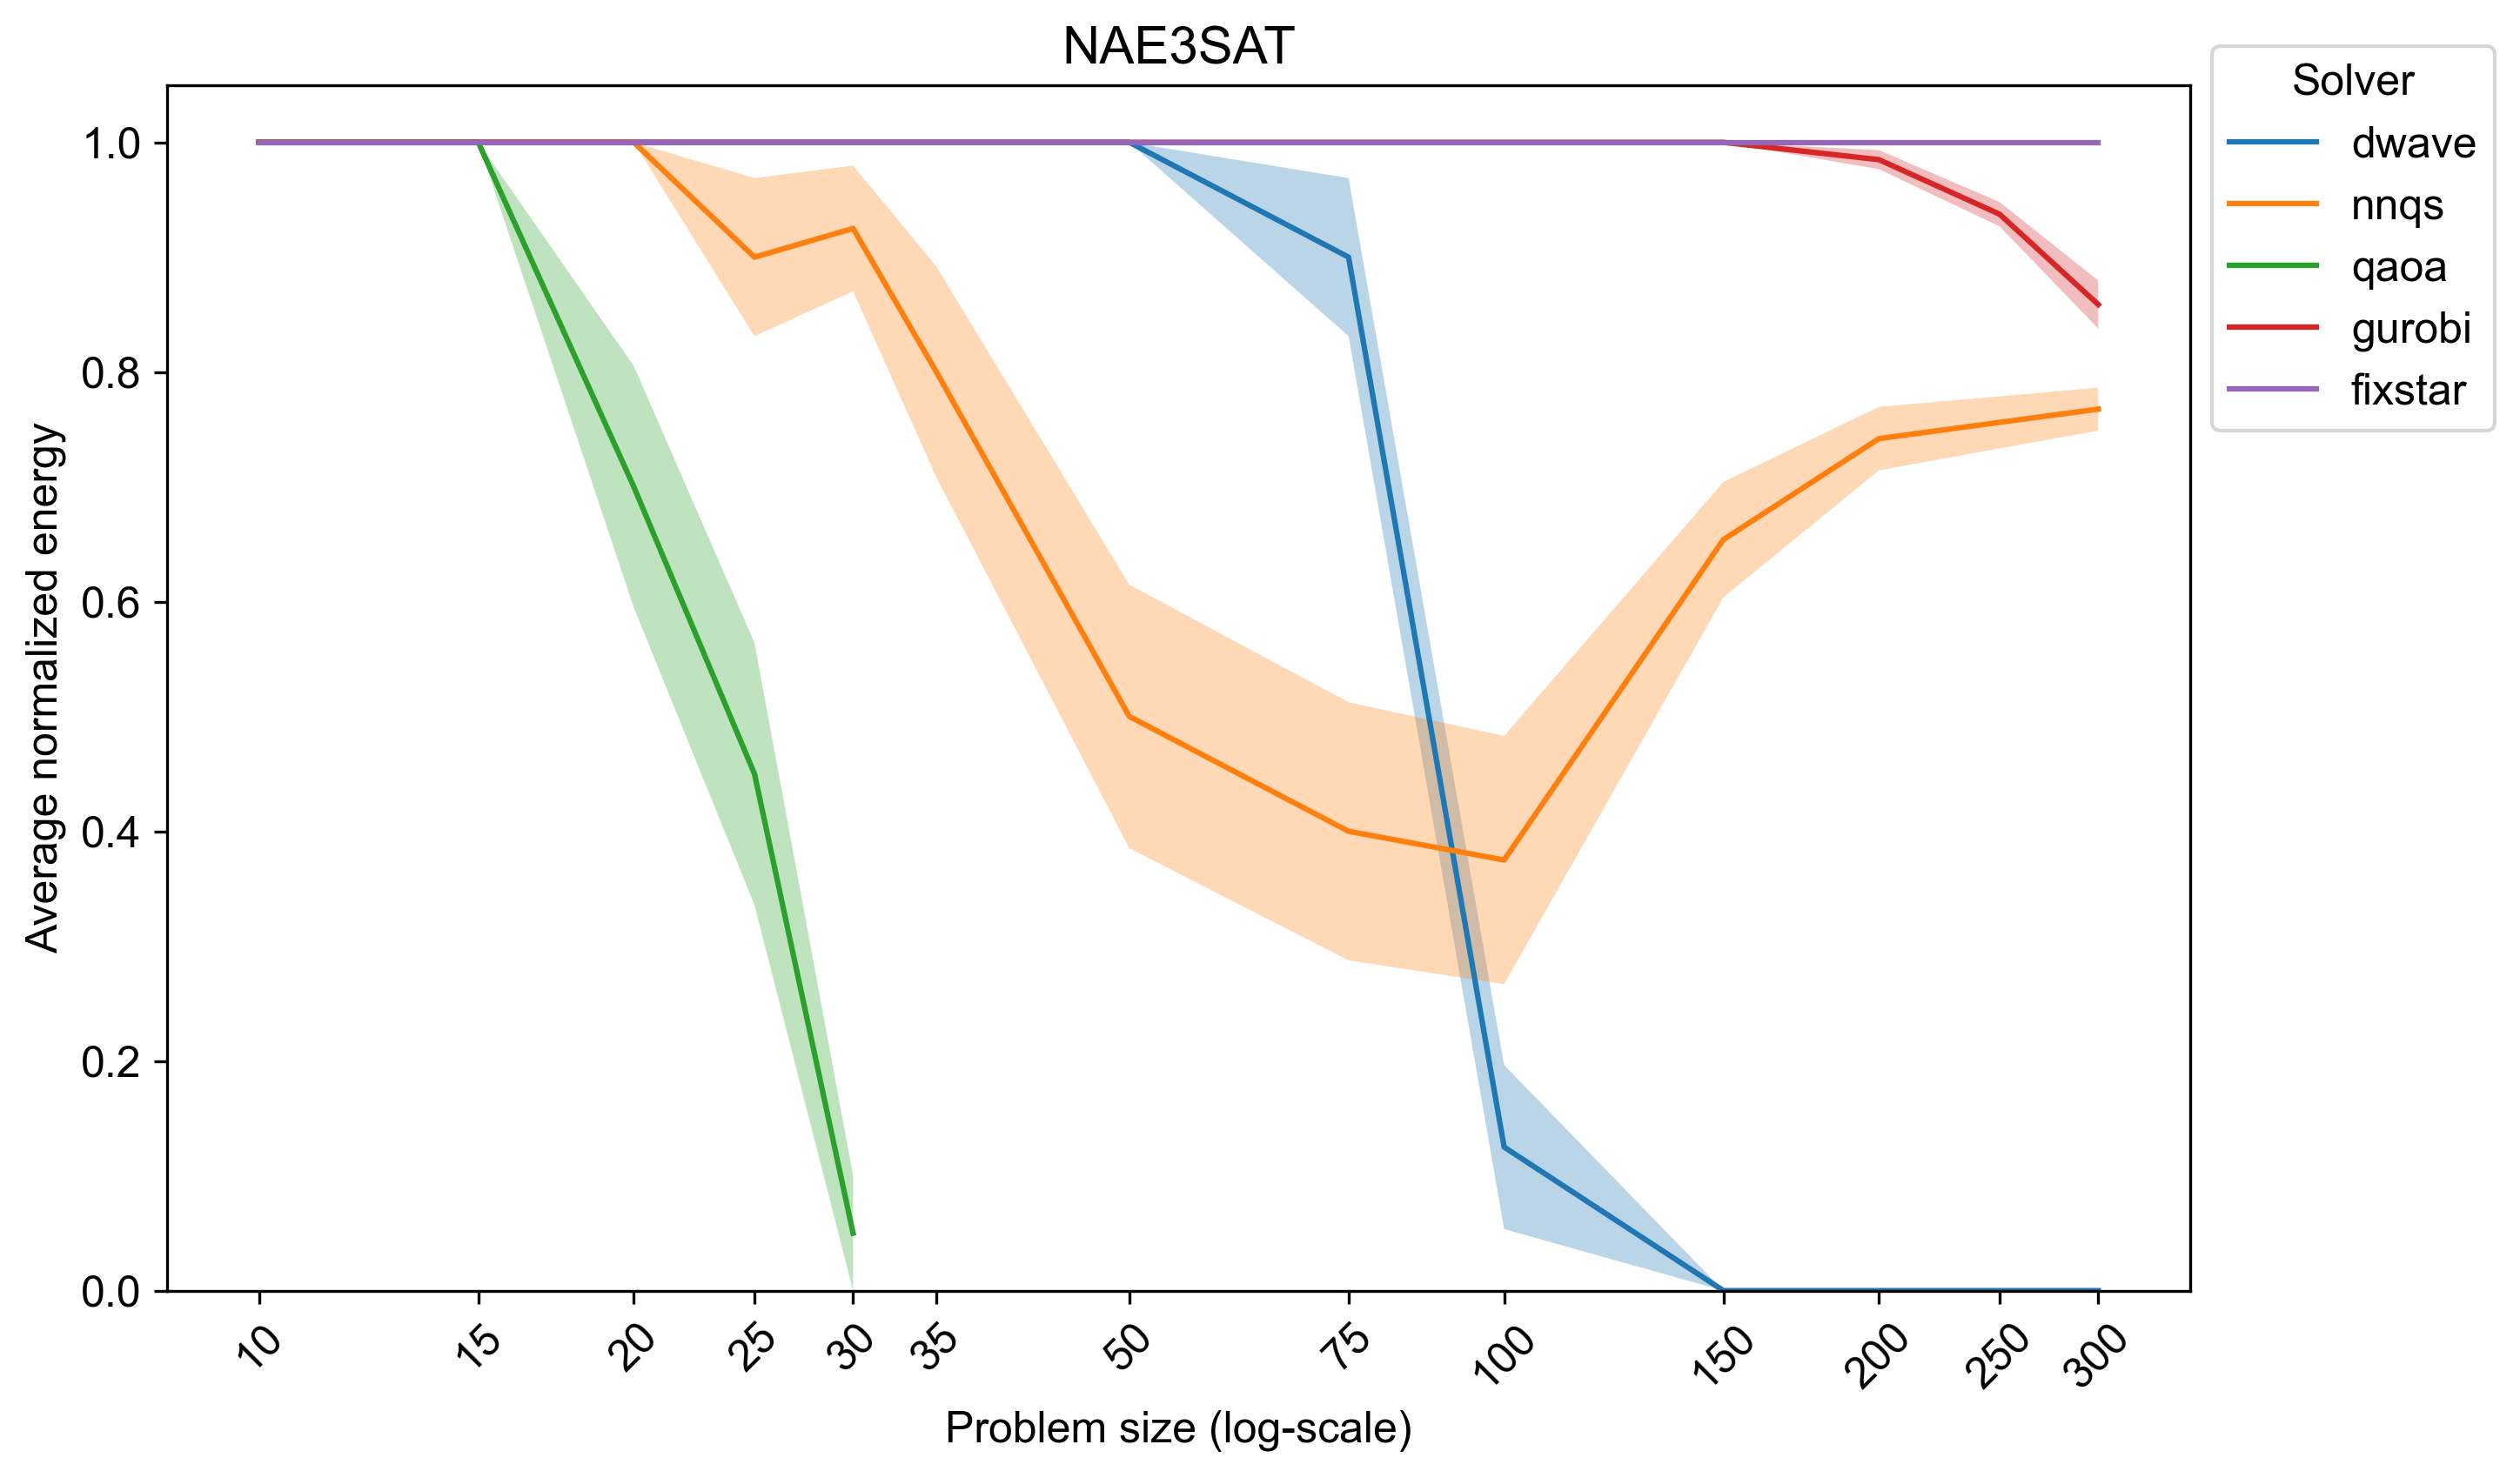
\includegraphics[width=0.9\textwidth]{images/nae3sat_all_size.png}}
    \\
    \subfloat[Success probability]{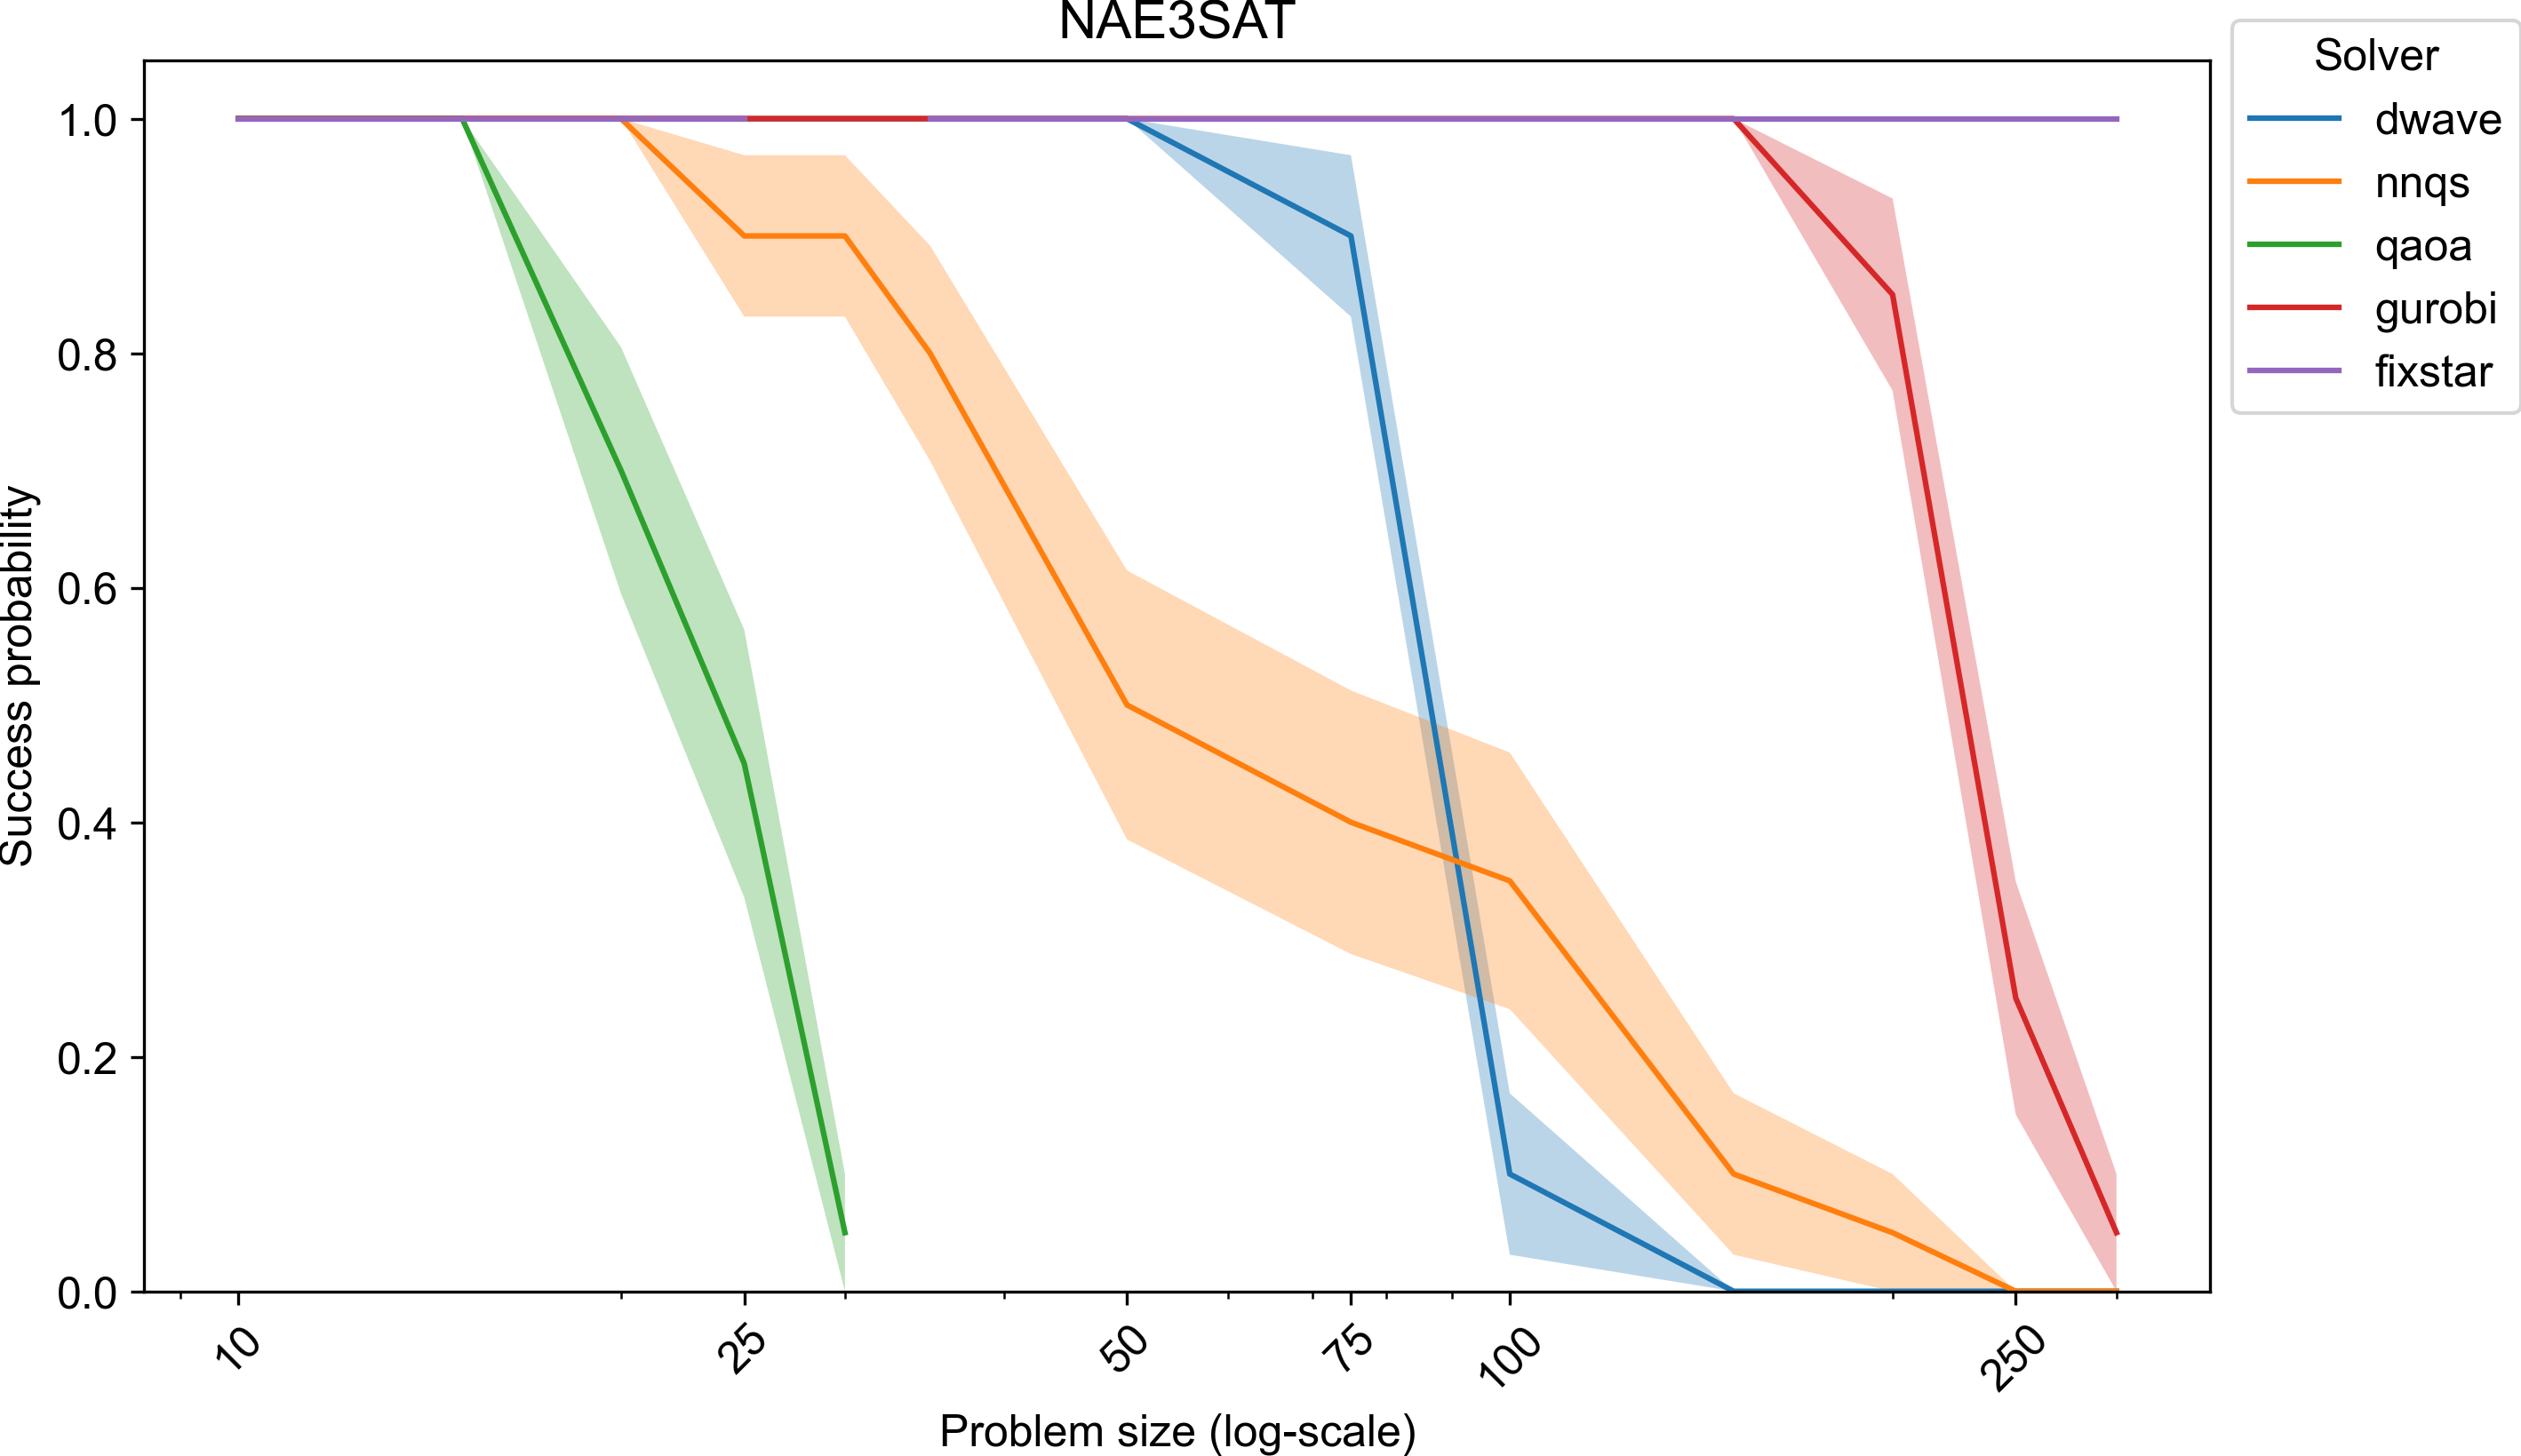
\includegraphics[width=0.9\textwidth]{images/nae3sat_all_success_size.png}}
    \caption{Performance of different solvers for NAE3SAT by problem size}
    \label{all-nae3sat-size}
\end{figure}

\begin{figure}[!htbp]
    \centering
    \subfloat[Normalized energy]{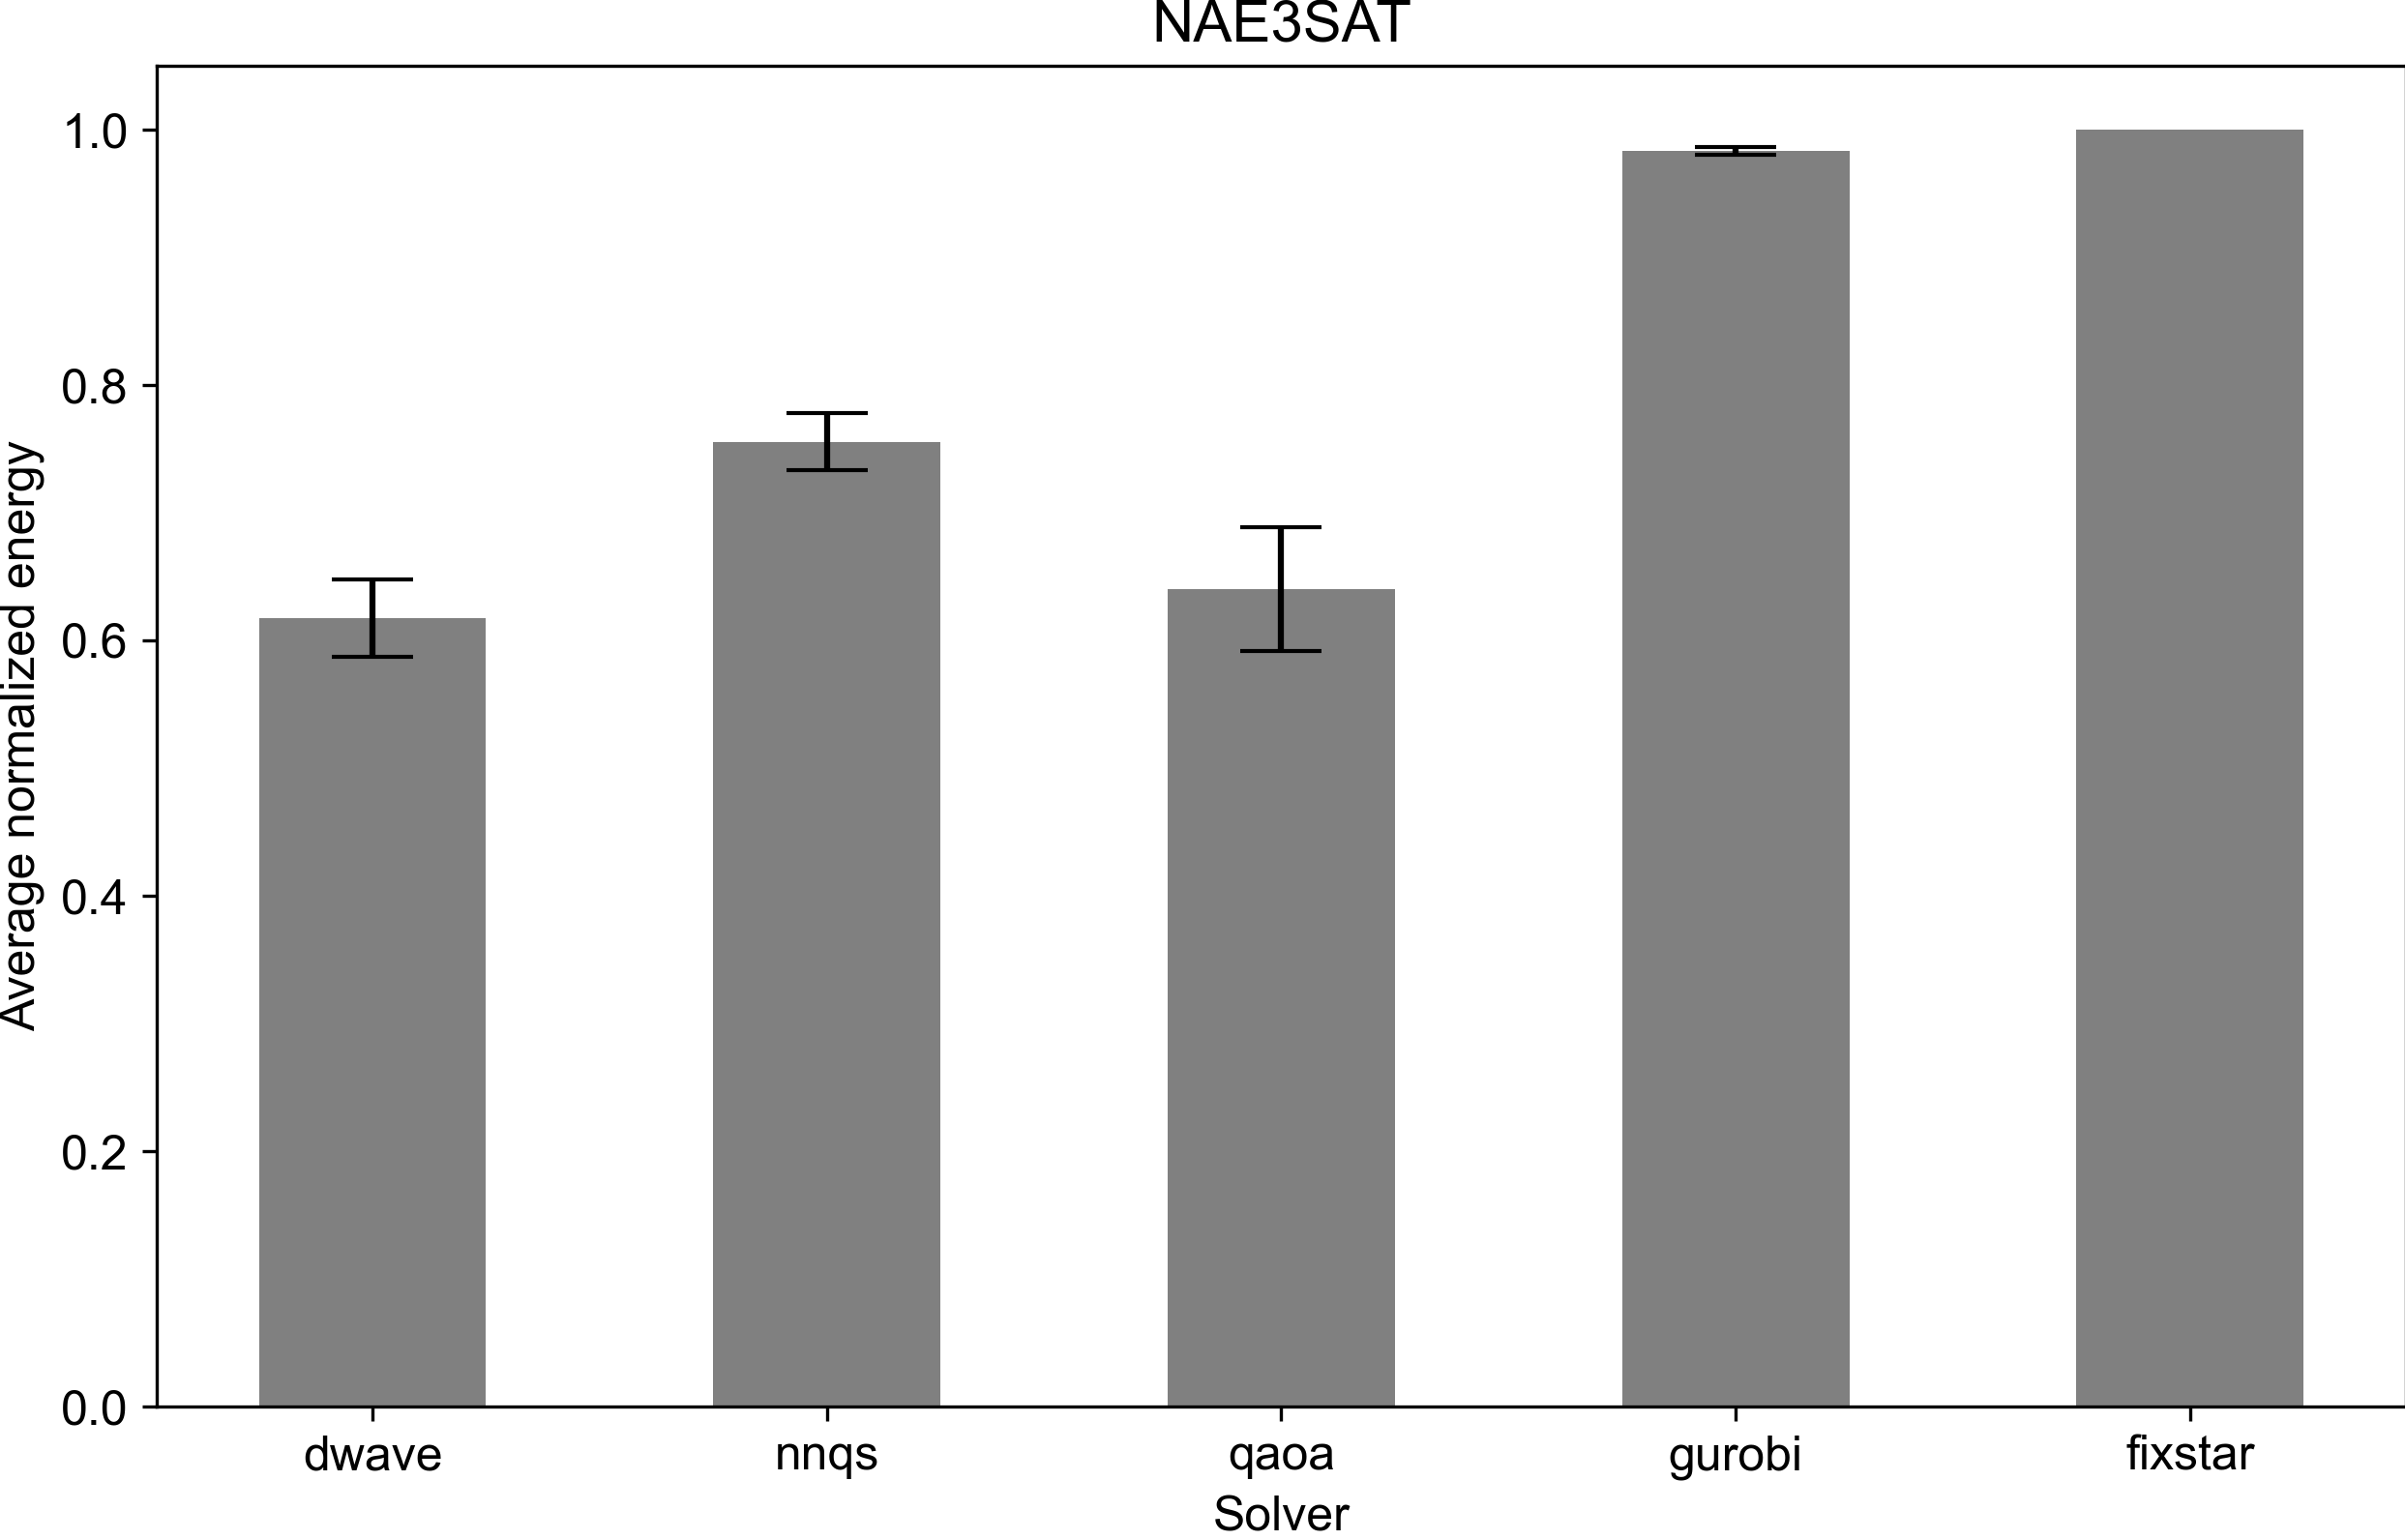
\includegraphics[width=0.49\textwidth]{images/nae3sat_all_avg.png}}\hfill
    \subfloat[Success probability]{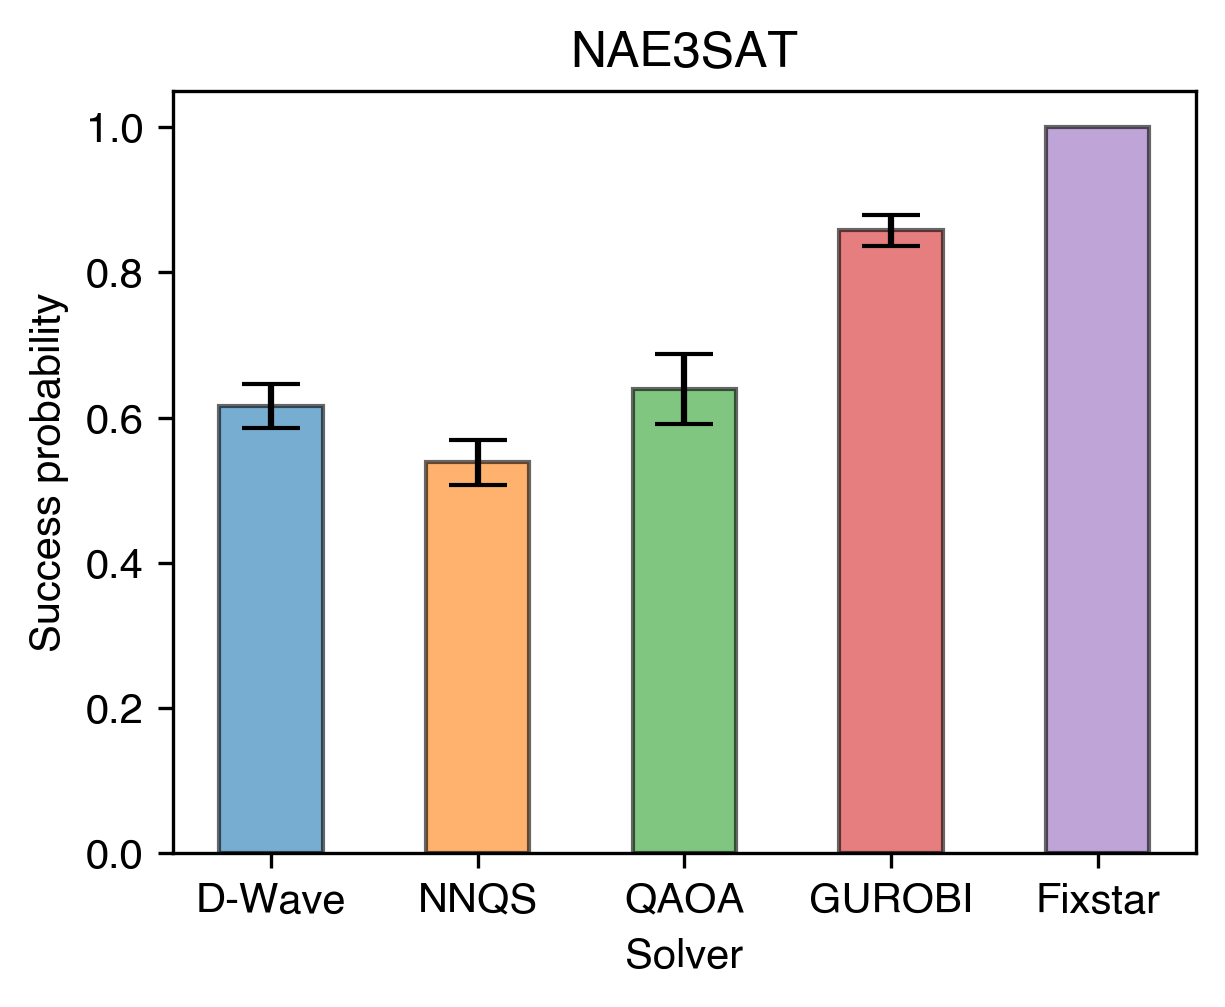
\includegraphics[width=0.49\textwidth]{images/nae3sat_all_success_avg.png}}
    \caption{Average performance of different solvers for NAE3SAT}
    \label{all-nae3sat-average}
\end{figure}

Performance by size for the NAE3SAT dataset in \autoref{all-nae3sat-size} and average performance is shown in \autoref{all-nae3sat-average}. The D-wave solver and NNQS could both solve problems up to $n=300$. However, multiple embedding requests were required for problems of size $300$ for the D-wave Pegasus topology which suggests that $n=300$ might be near the D-wave size limit for the NAE3SAT problem. QAOA was only able to solve problems of up to $n=30$ due to the limitations on the number of qubits of the simulator.

In terms of performance, the D-wave solver performs well up to $n=50$ with a success probability of $1$. For larger problem sizes, the performance of the D-wave solver drops off sharply. The NNQS performs well up to $n=20$, and then the success probability and normalized energy gradually decline until $n=300$. The QAOA solver performs well up to $n=15$, with declining performance until $n=30$. Between the classical solvers, the Fixstars QUBO solver performs better than the GUROBI optimizer at larger problem sizes ($>150$).

Overall, the NNQS has the highest average normalized energy among the 3 quantum-inspired solvers but has the lowest success probability. This is likely due to it being able to solve problems of larger sizes that the D-wave Annealer and QAOA solver cannot handle.

\subsection{Max-cut}

\begin{figure}[!htbp]
    \centering
    \subfloat[Normalized energy]{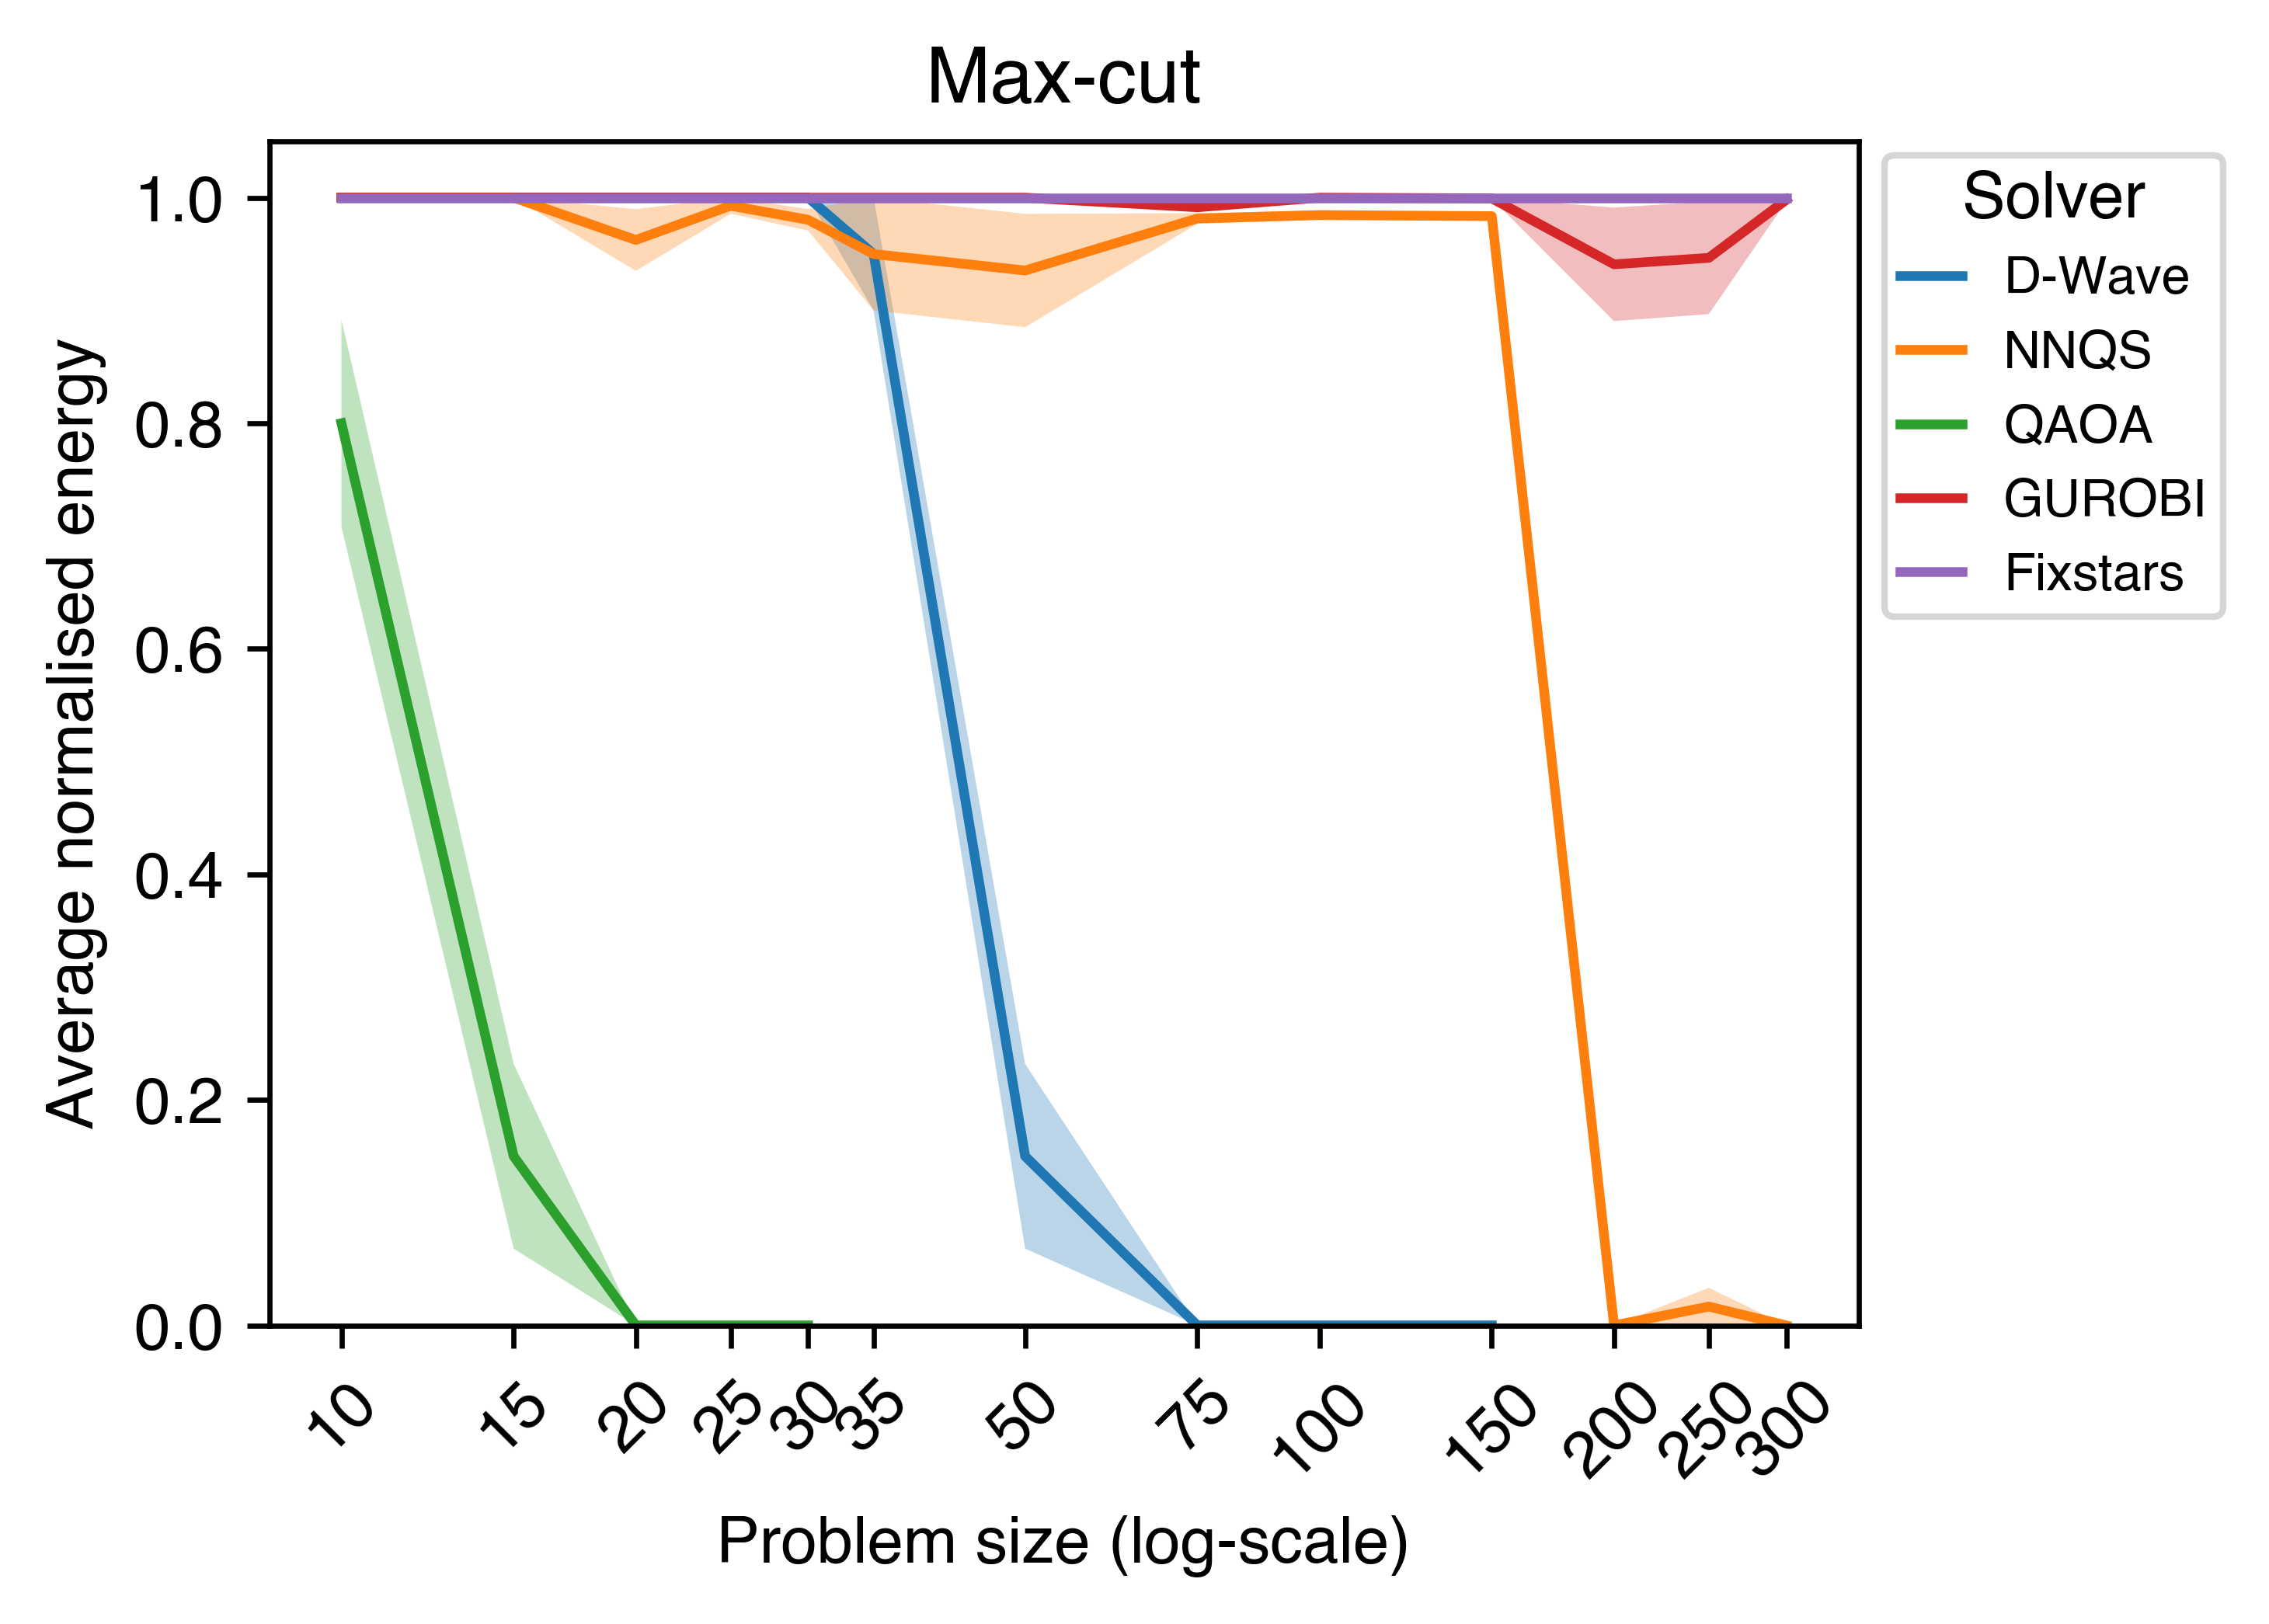
\includegraphics[width=0.9\textwidth]{images/maxcut_all_size.png}}
    \\
    \subfloat[Success probability]{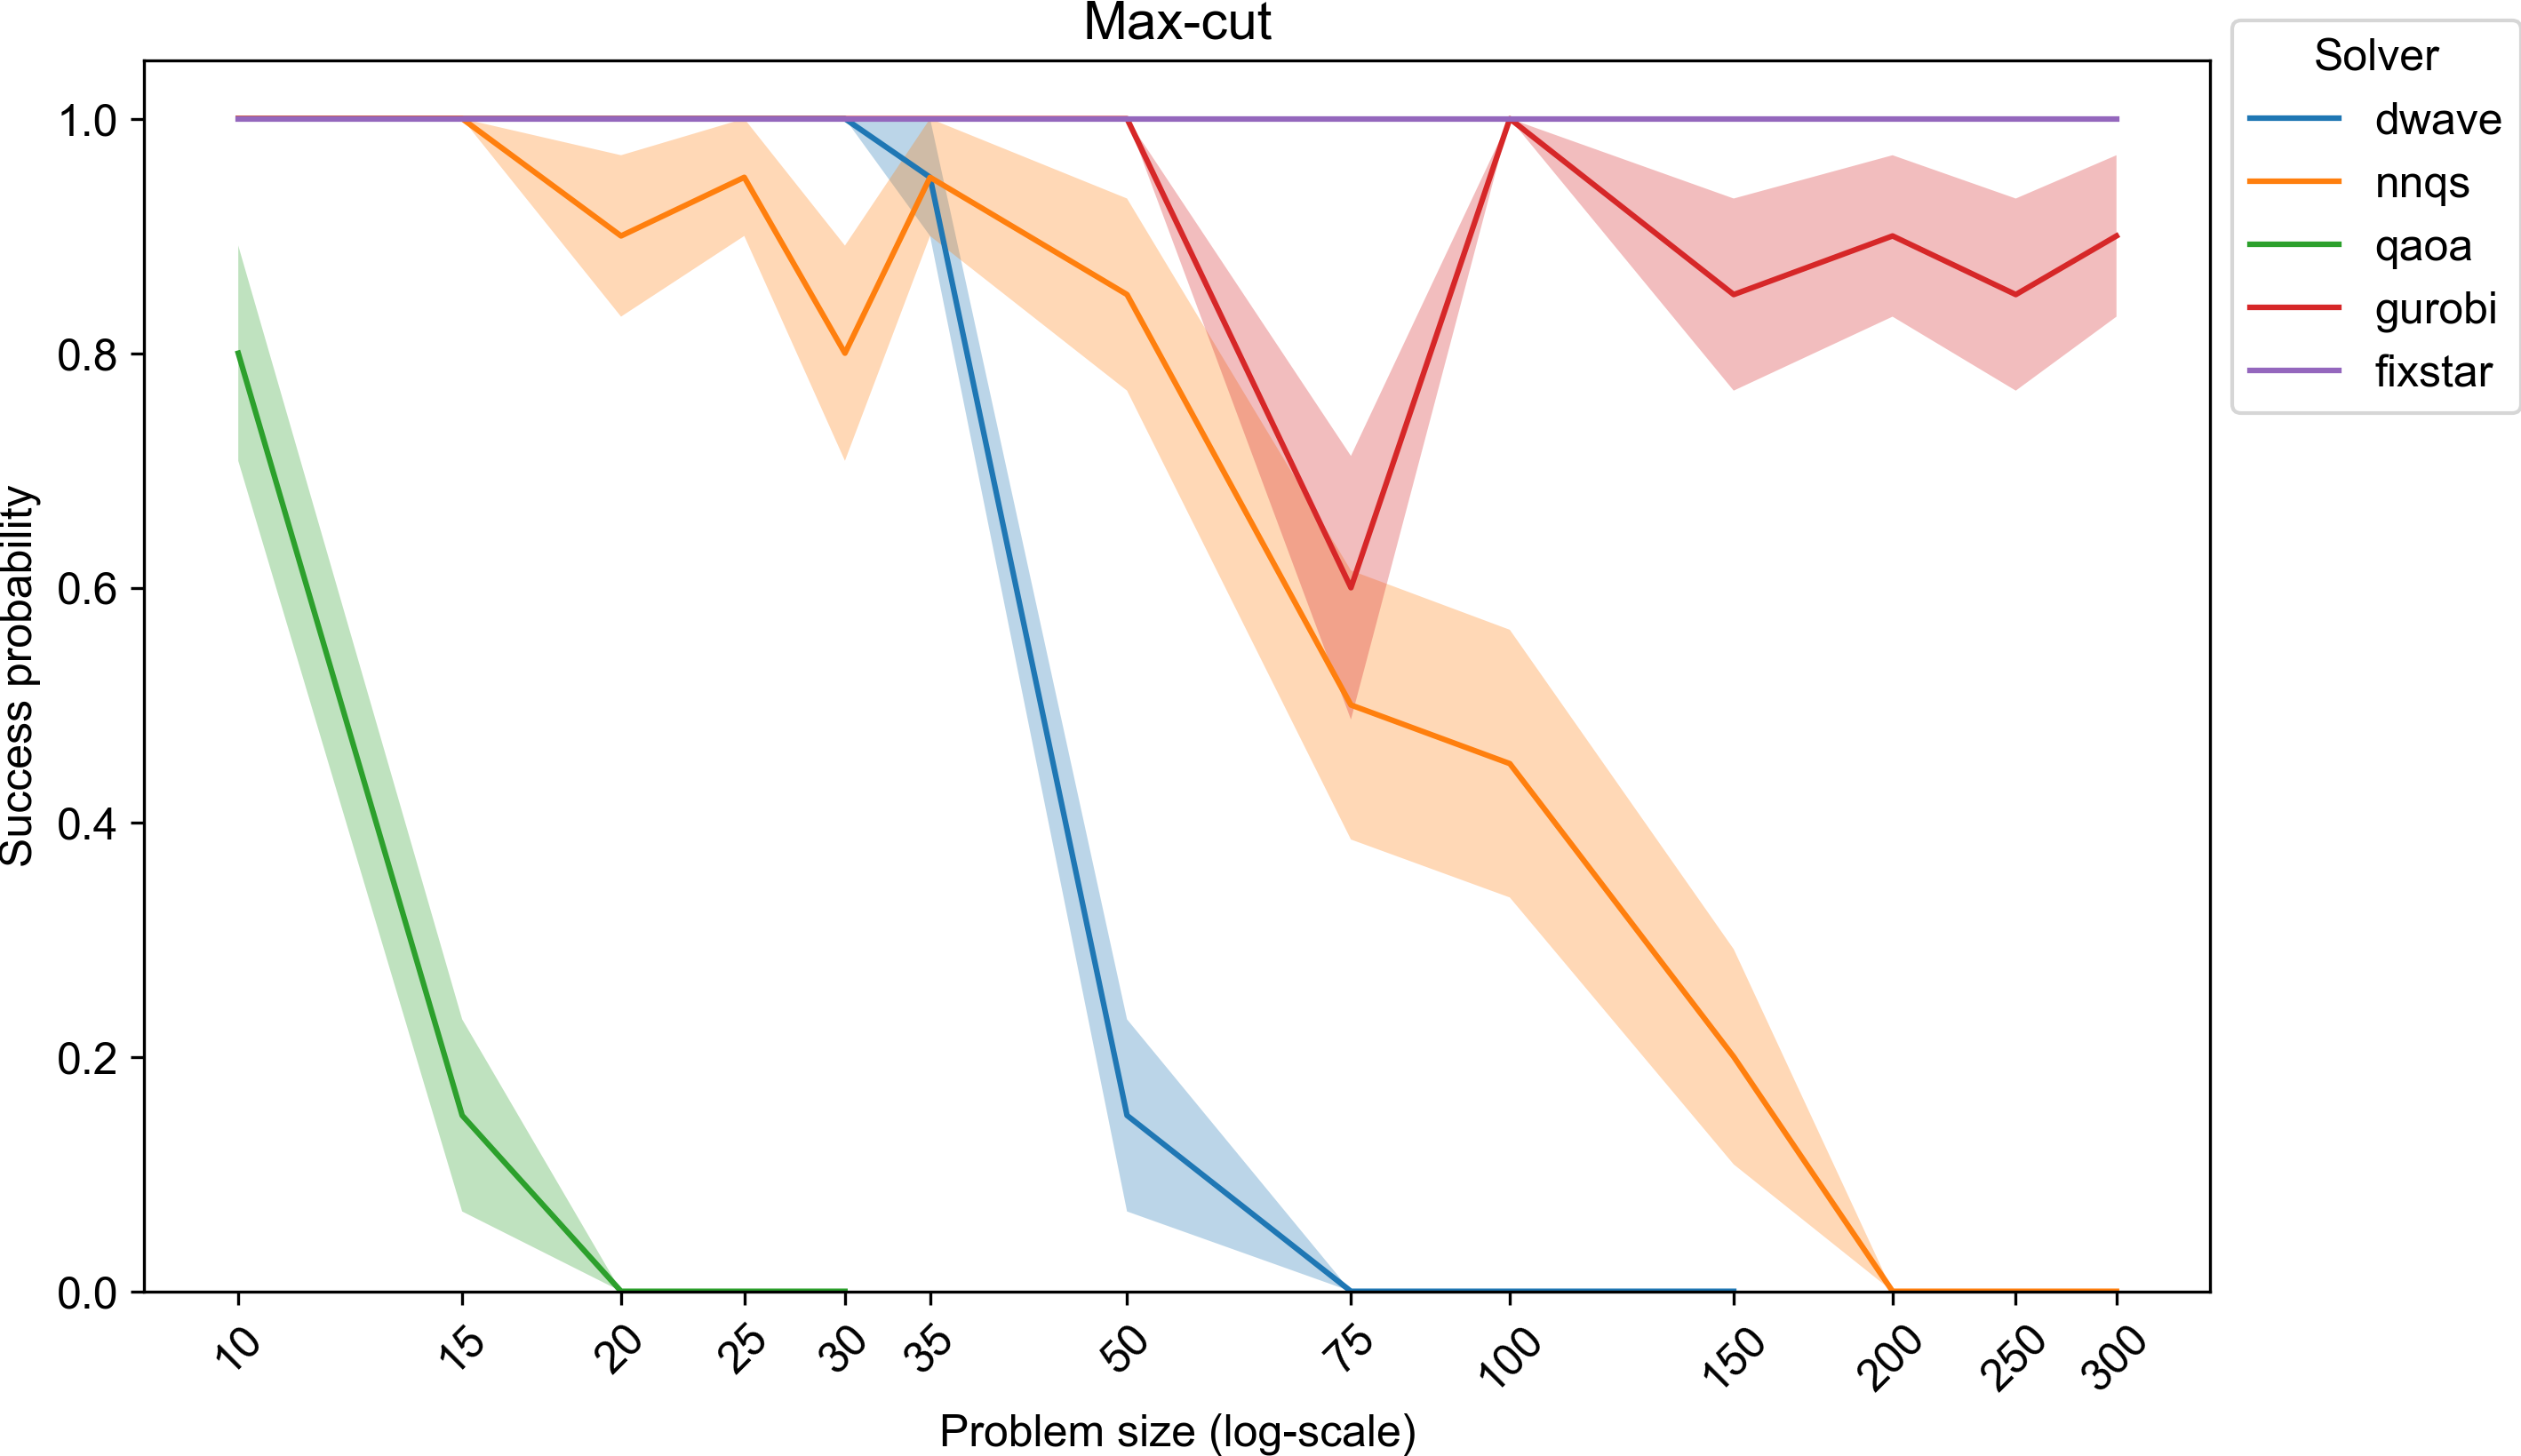
\includegraphics[width=0.9\textwidth]{images/maxcut_all_success_size.png}}
    \caption{Performance of different solvers for max-cut by problem size}
    \label{all-maxcut-size}
\end{figure}

\begin{figure}[!htbp]
    \centering
    \subfloat[Normalized energy]{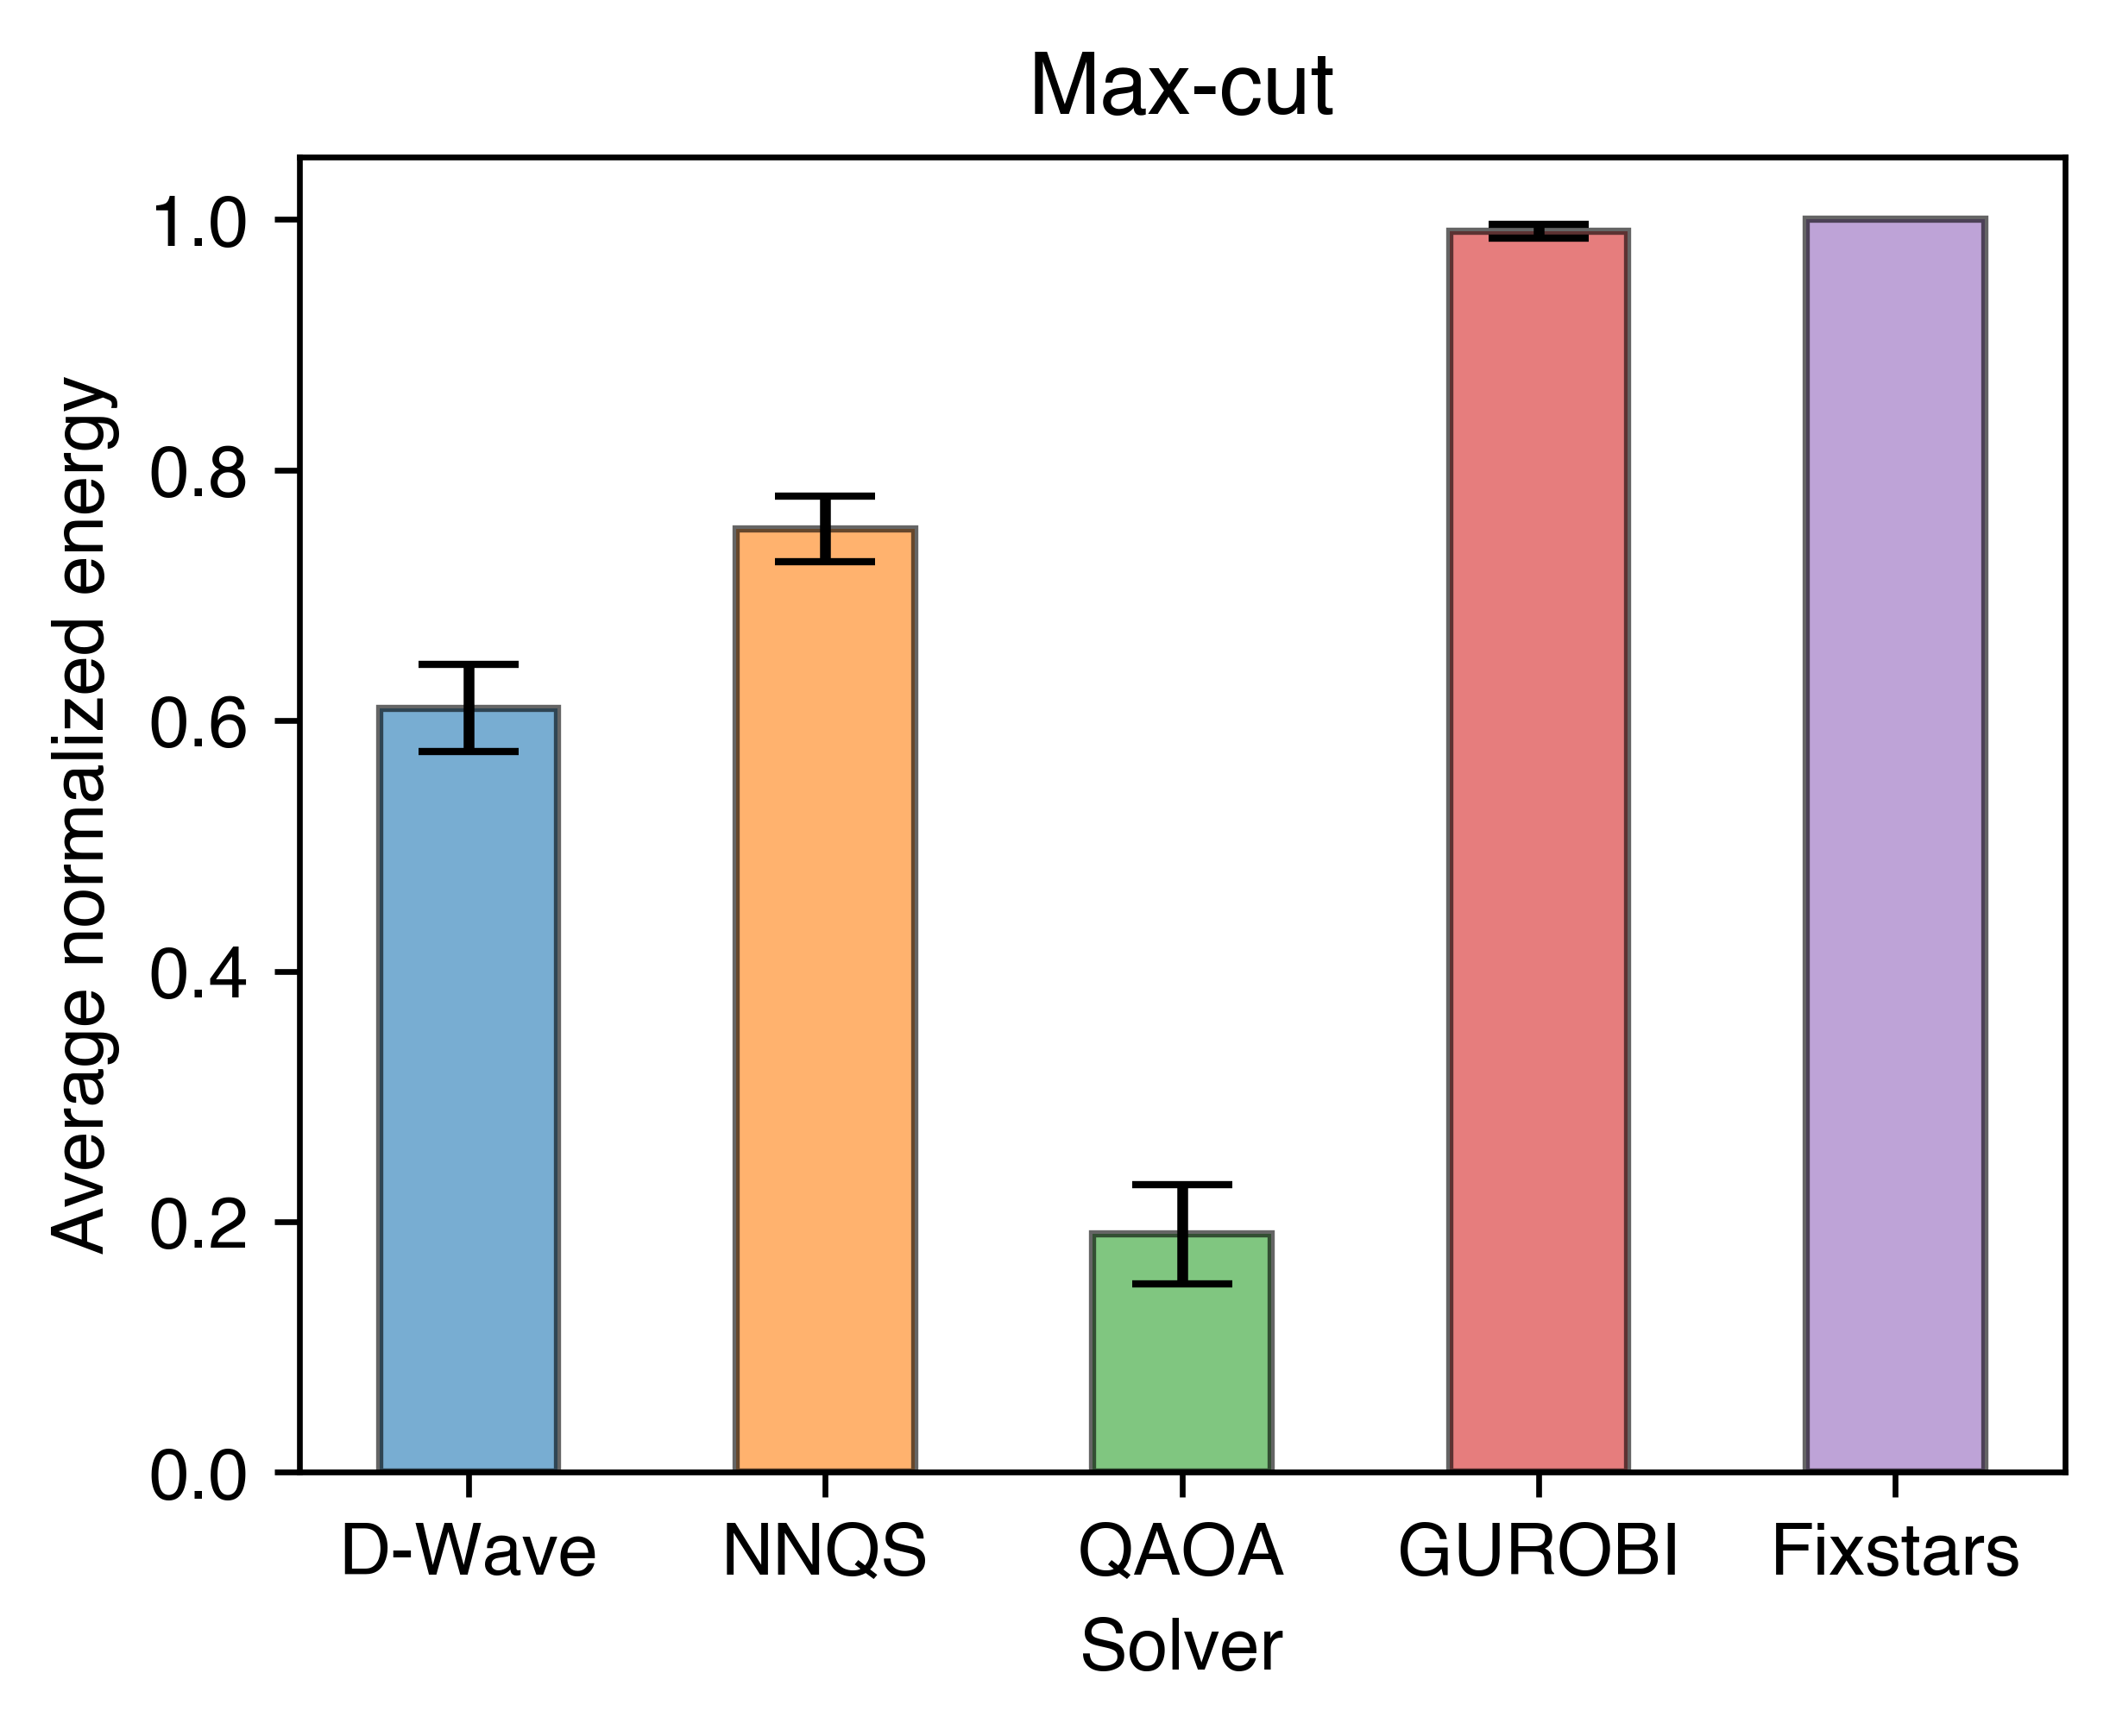
\includegraphics[width=0.49\textwidth]{images/maxcut_all_avg.png}}\hfill
    \subfloat[Success probability]{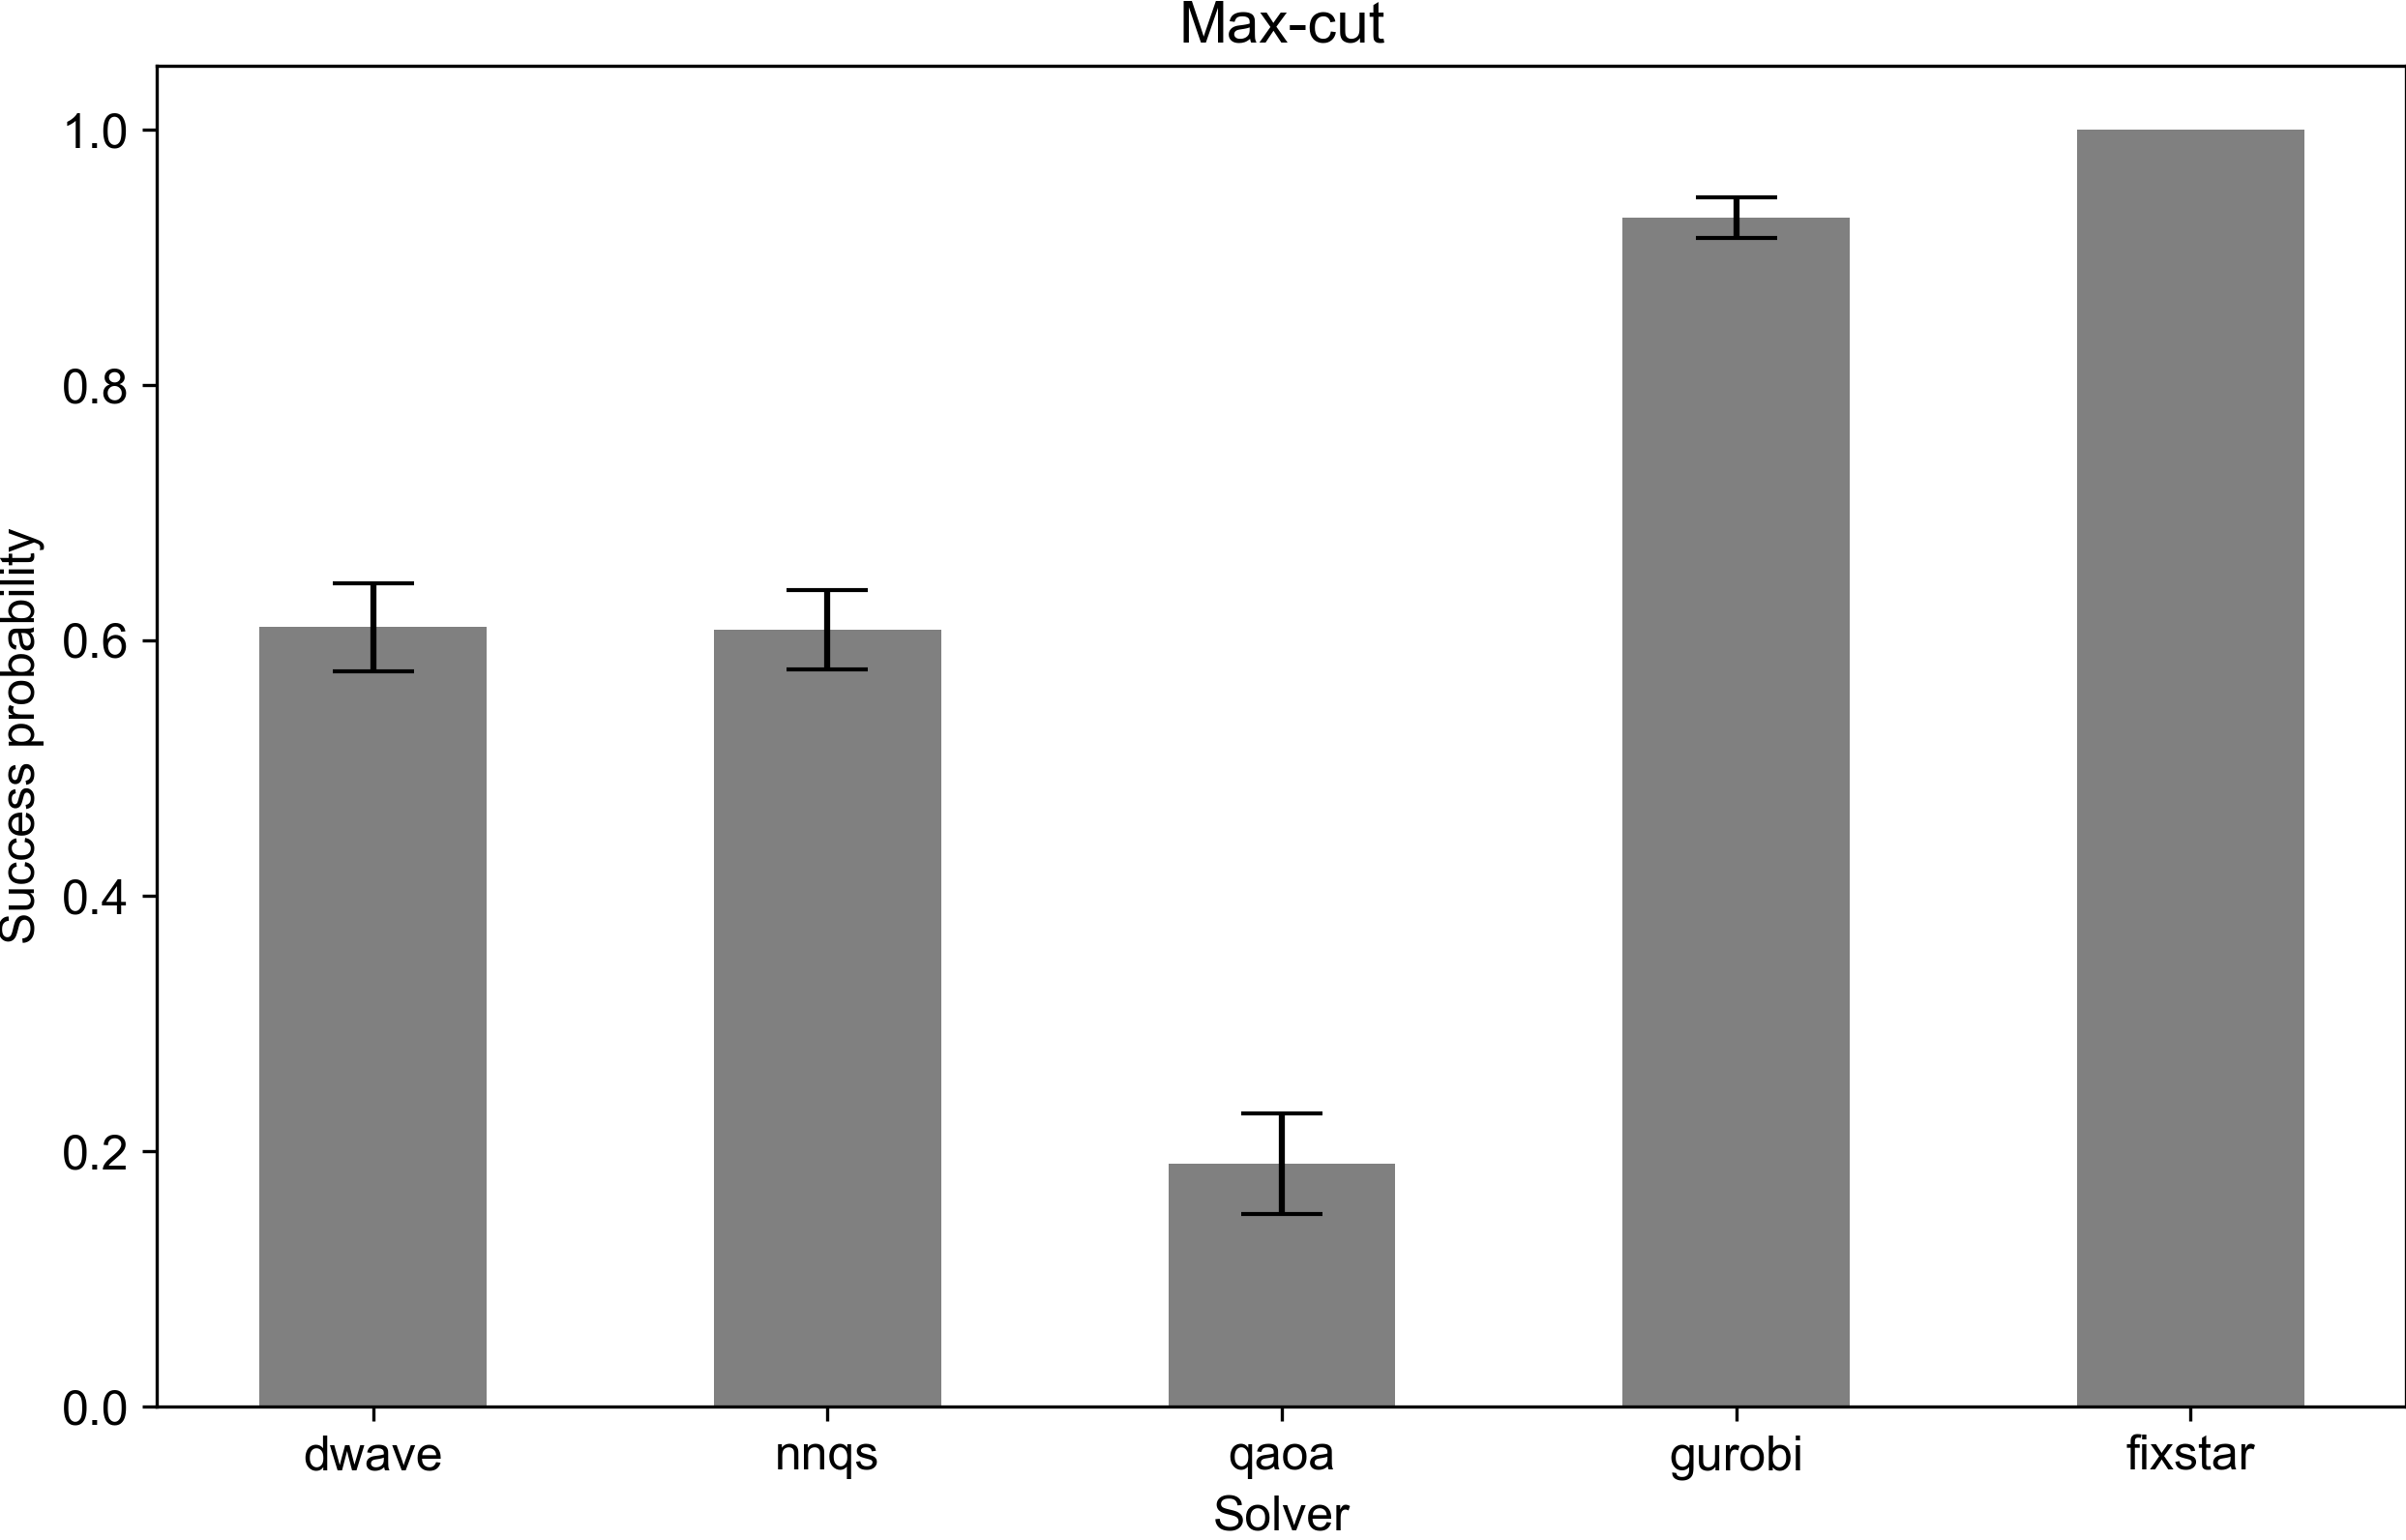
\includegraphics[width=0.49\textwidth]{images/maxcut_all_success_avg.png}}
    \caption{Average performance of different solvers for max-cut}
    \label{all-maxcut-average}
\end{figure}

Performance by size for the max-cut dataset is shown in \autoref{all-maxcut-size} and average performance is shown in \autoref{all-maxcut-average}. For the max-cut problem, the D-wave solver could only handle problem sizes up to $n=150$ due to the need for minor embedding onto the pegasus topology. QAOA was able to solve problems of up to $n=30$ due to the limitations of the simulator.

In terms of performance, the D-wave solver performs well up to $n=30$ and the performance drops off sharply for larger problems. The NNQS performs well up to $n=150$, although the success probability declines for sizes more than $50$. The QAOA solver performs well only for $n=10$, with performance declining afterward.

Overall, the NNQS has the highest average normalized energy among the 3 quantum-inspired solvers and has similar a success probability as the D-wave solver. The QAOA solver performs poorly in both metrics.

\subsection{SK model}

\begin{figure}[!htbp]
    \centering
    \subfloat[Normalized energy]{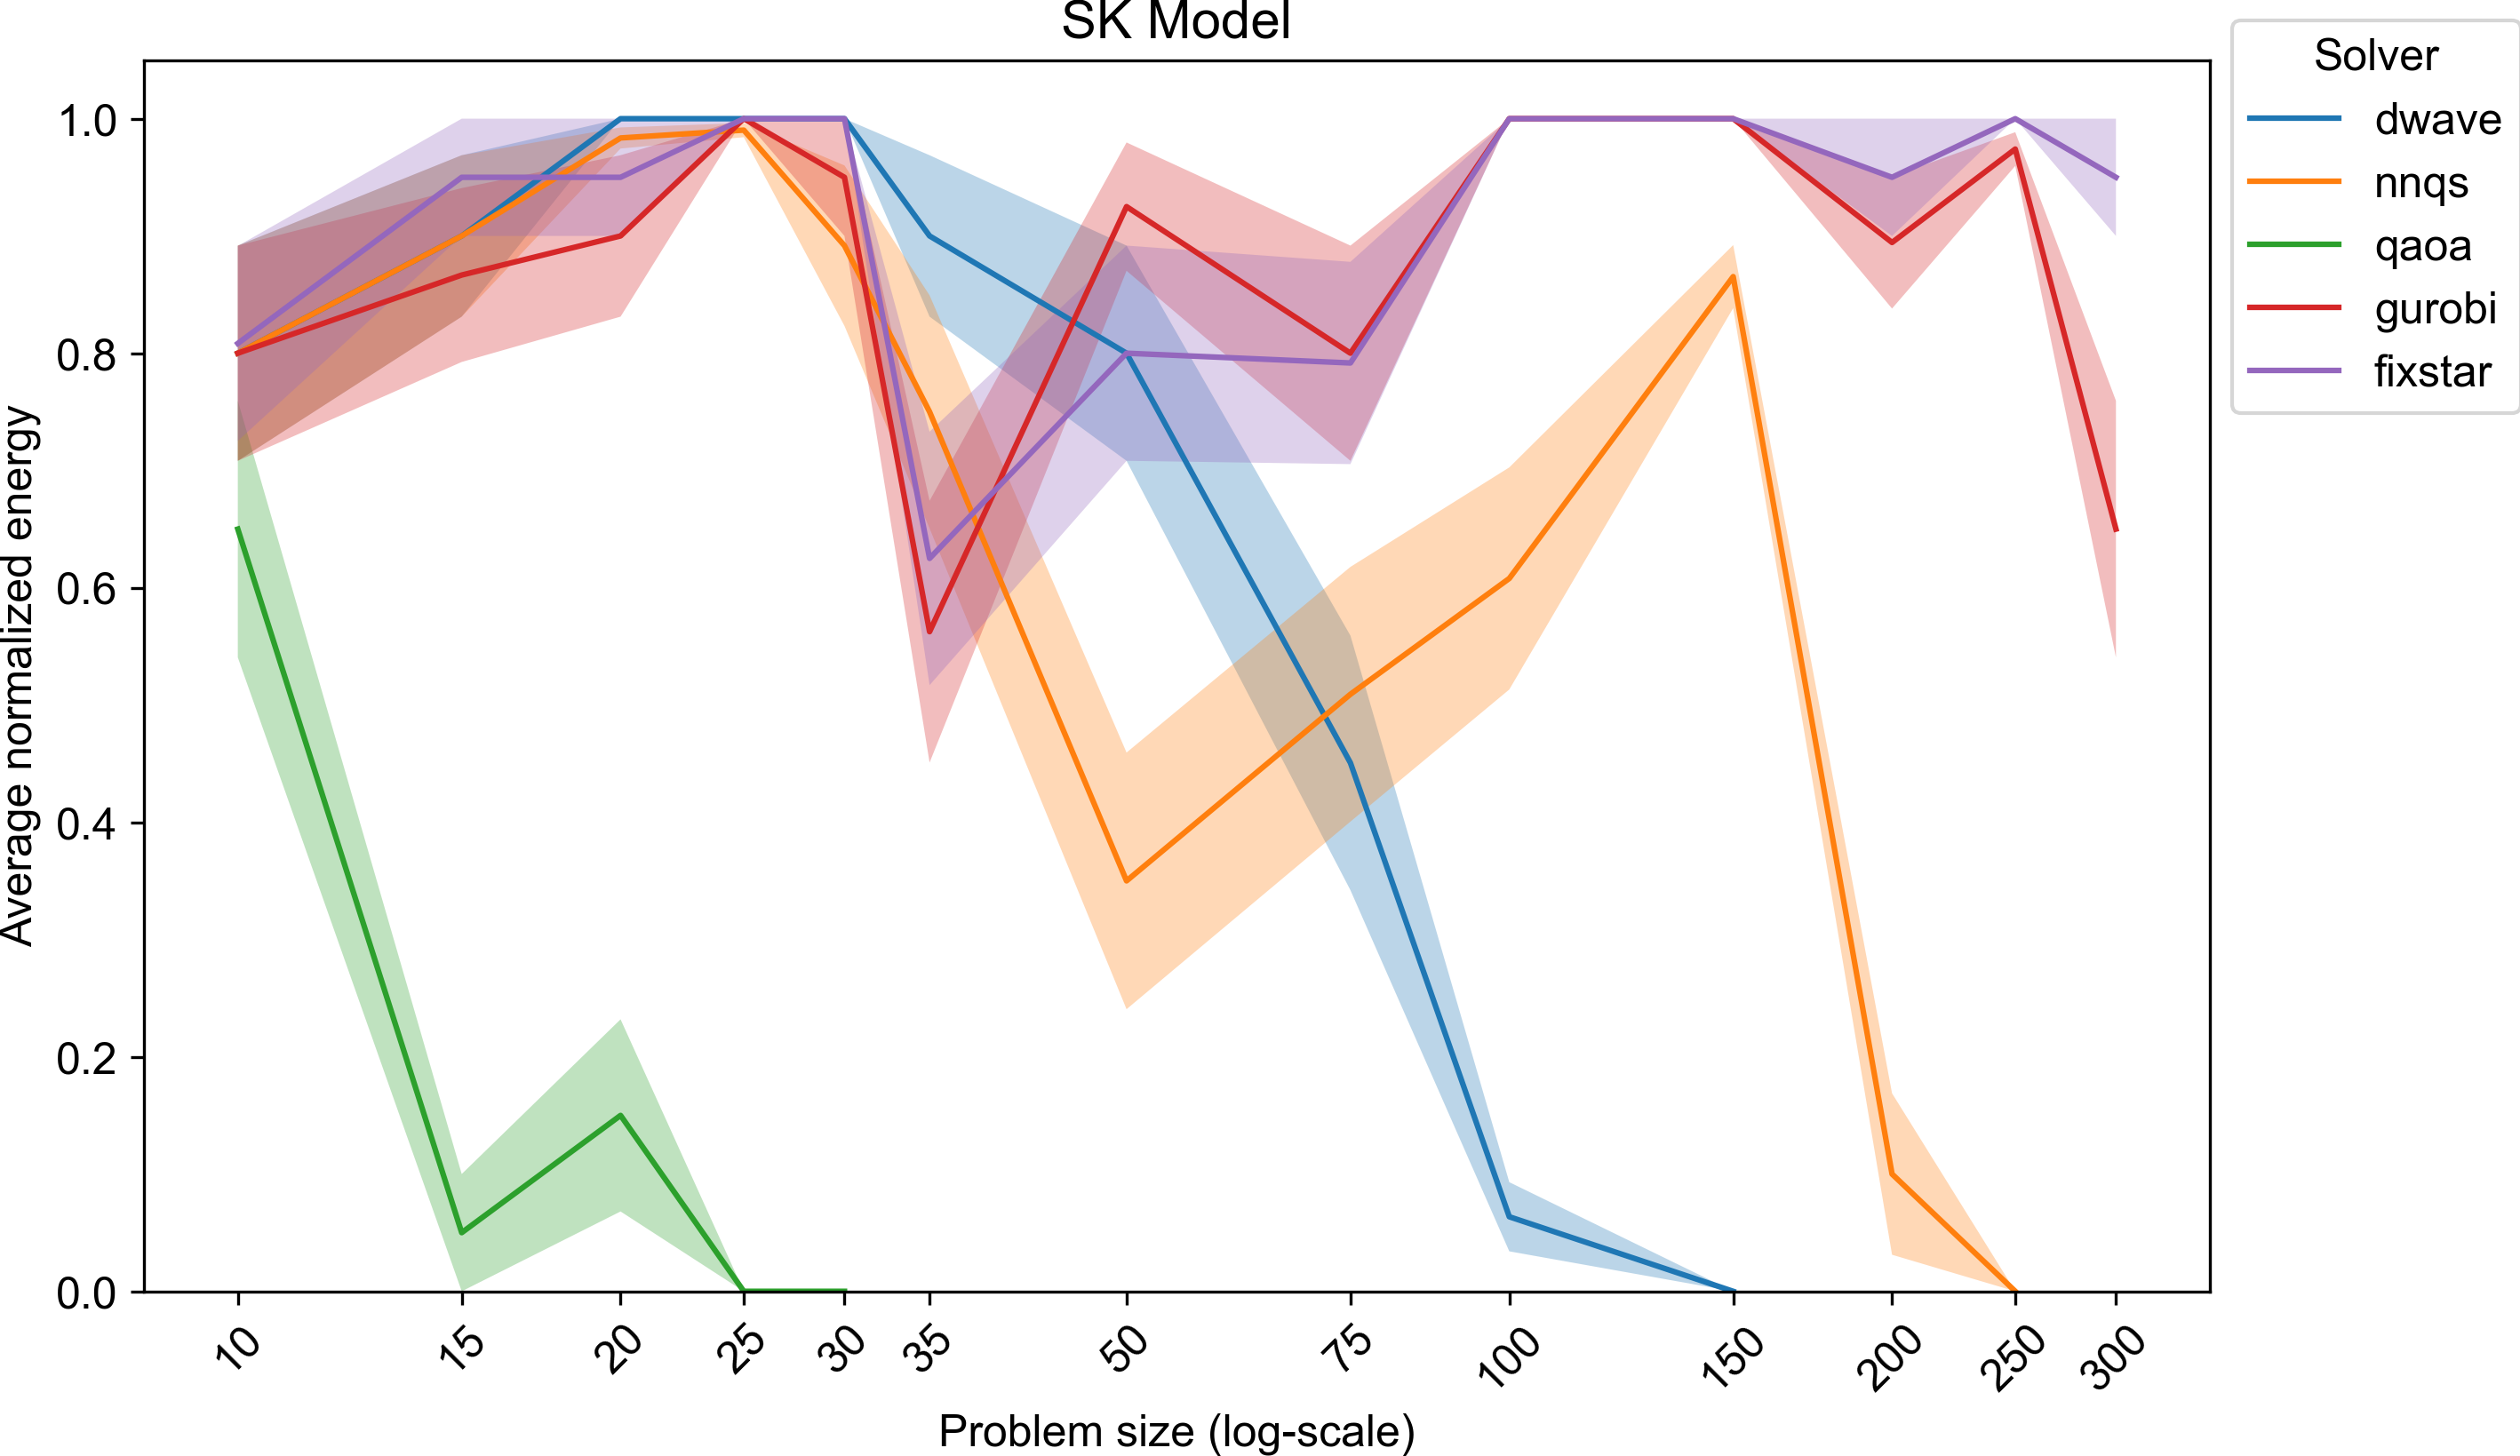
\includegraphics[width=0.9\textwidth]{images/skmodel_all_size.png}}%\hfill
    \\
    \subfloat[Success probability]{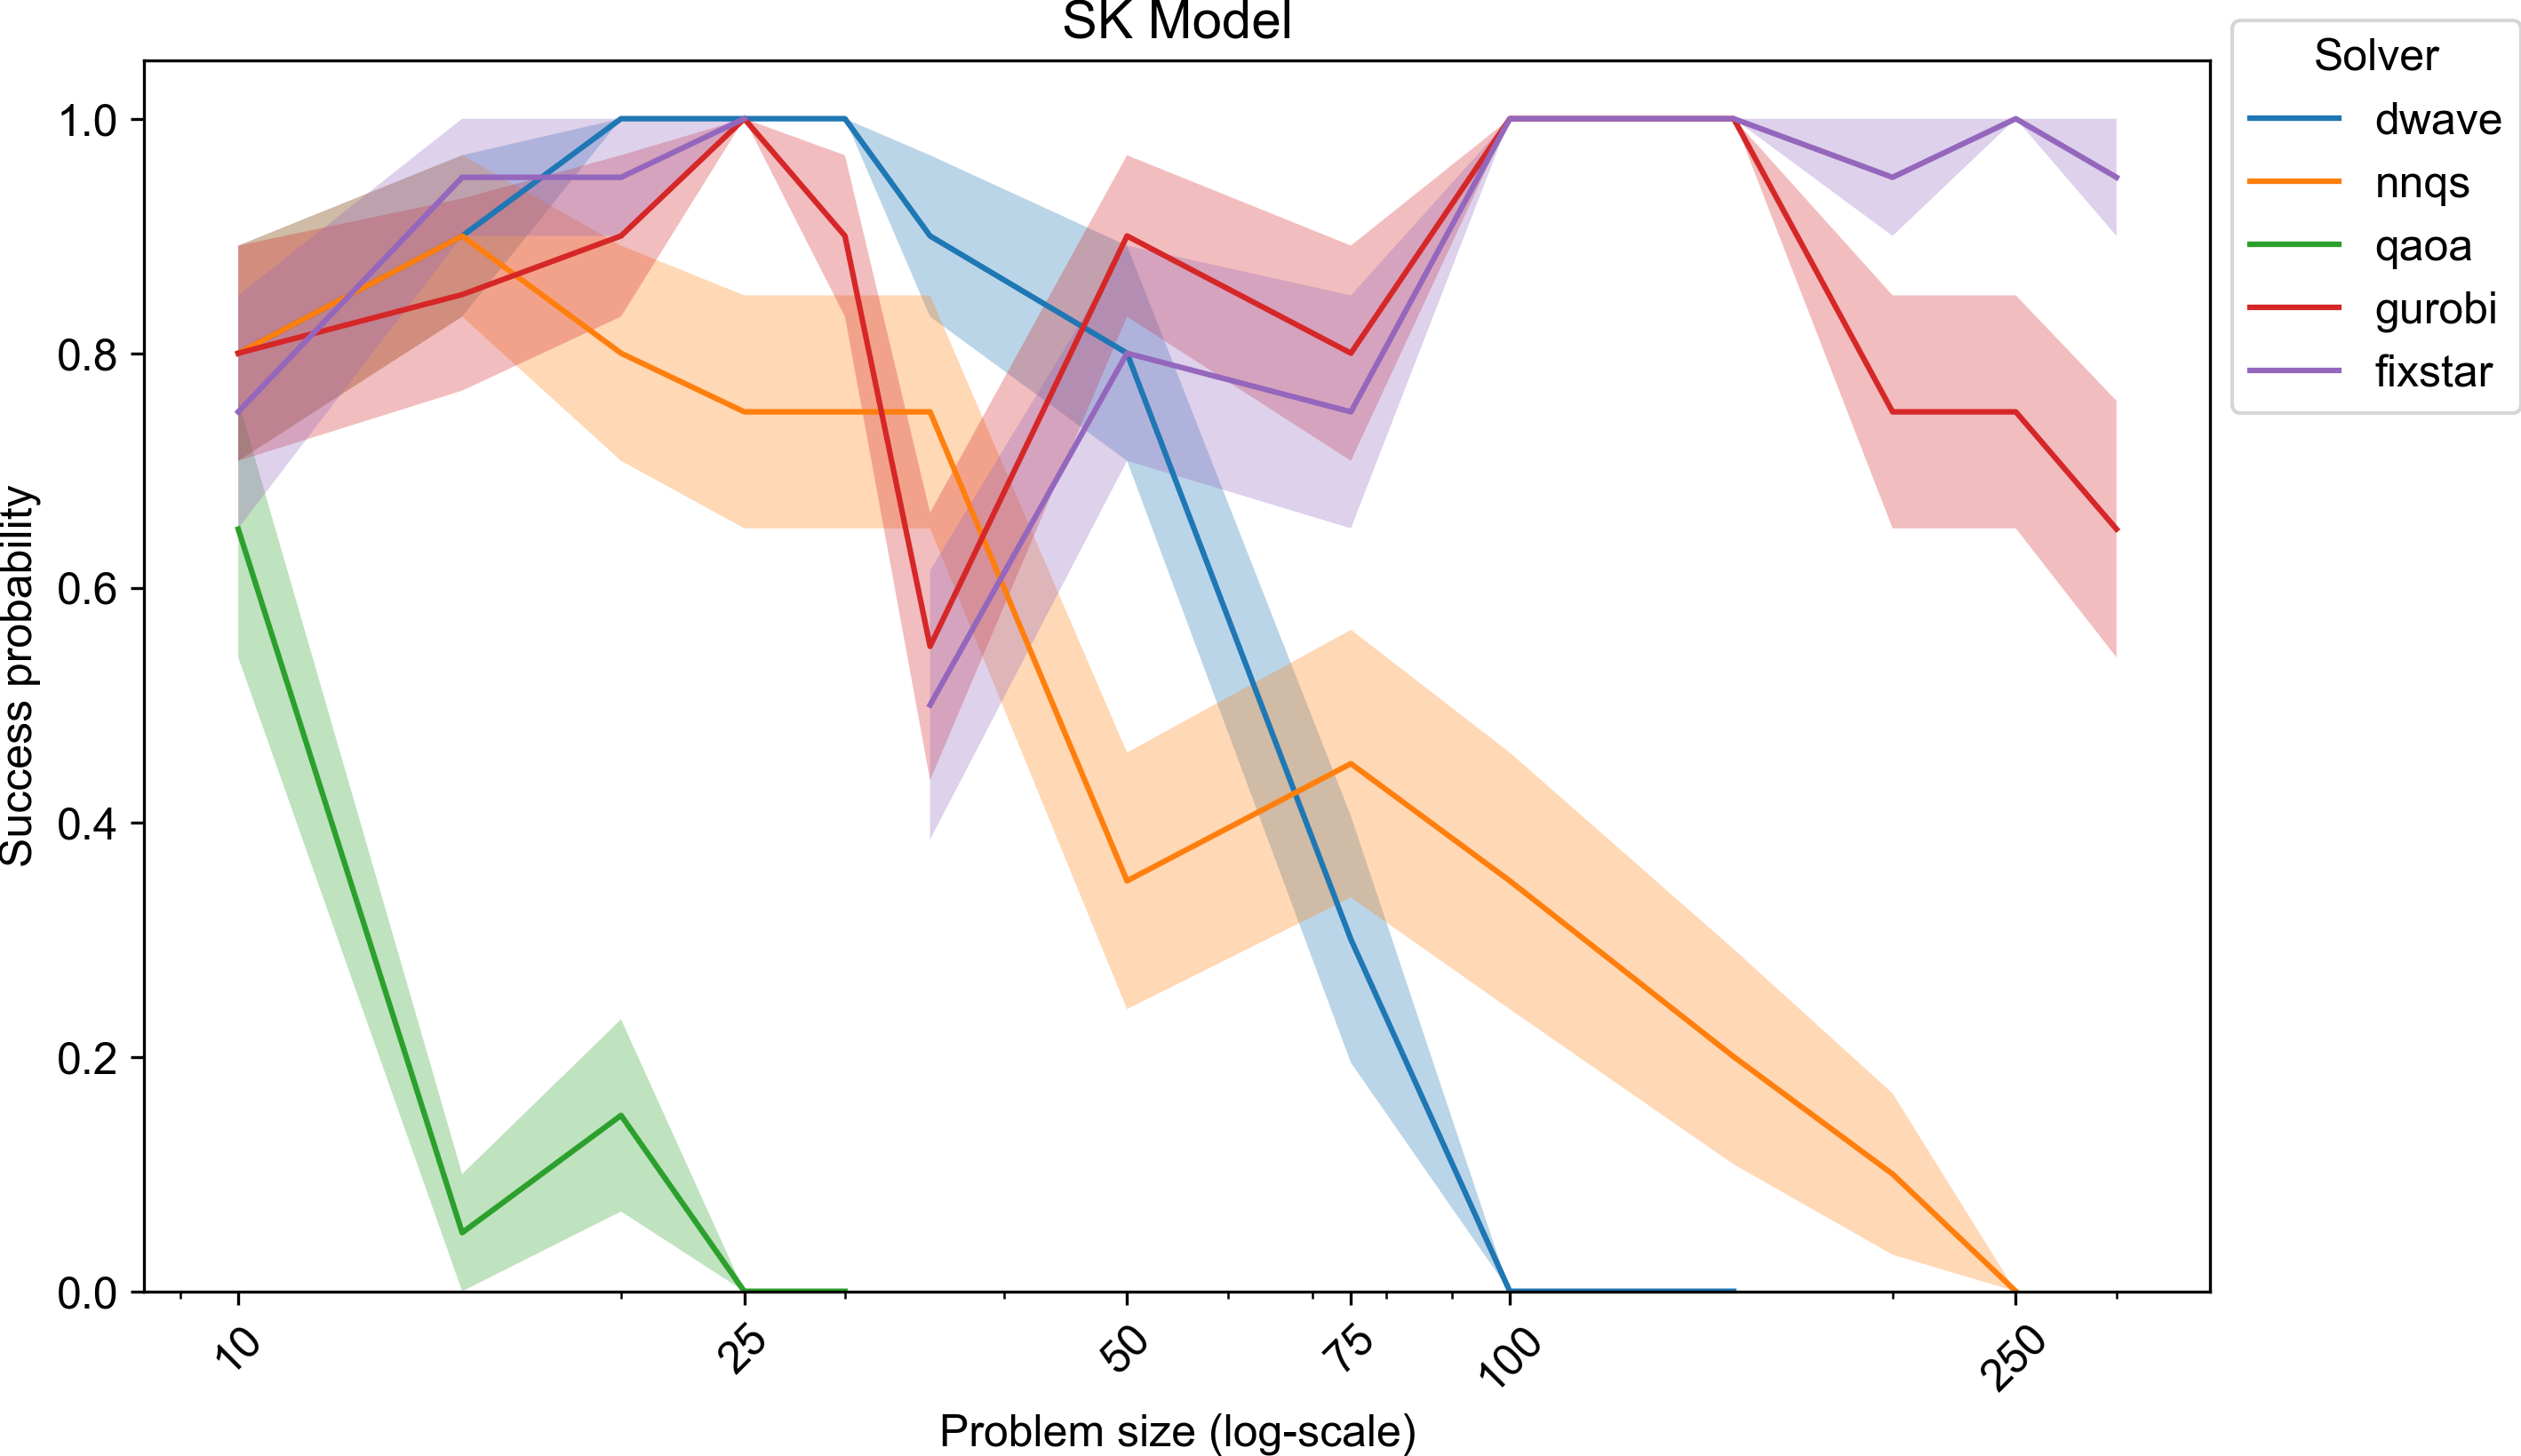
\includegraphics[width=0.9\textwidth]{images/skmodel_all_success_size.png}}
    \caption{Performance of different solvers for SK model by problem size}
    \label{all-skmodel-size}
\end{figure}

\begin{figure}[!htbp]
    \centering
    \subfloat[Normalized energy]{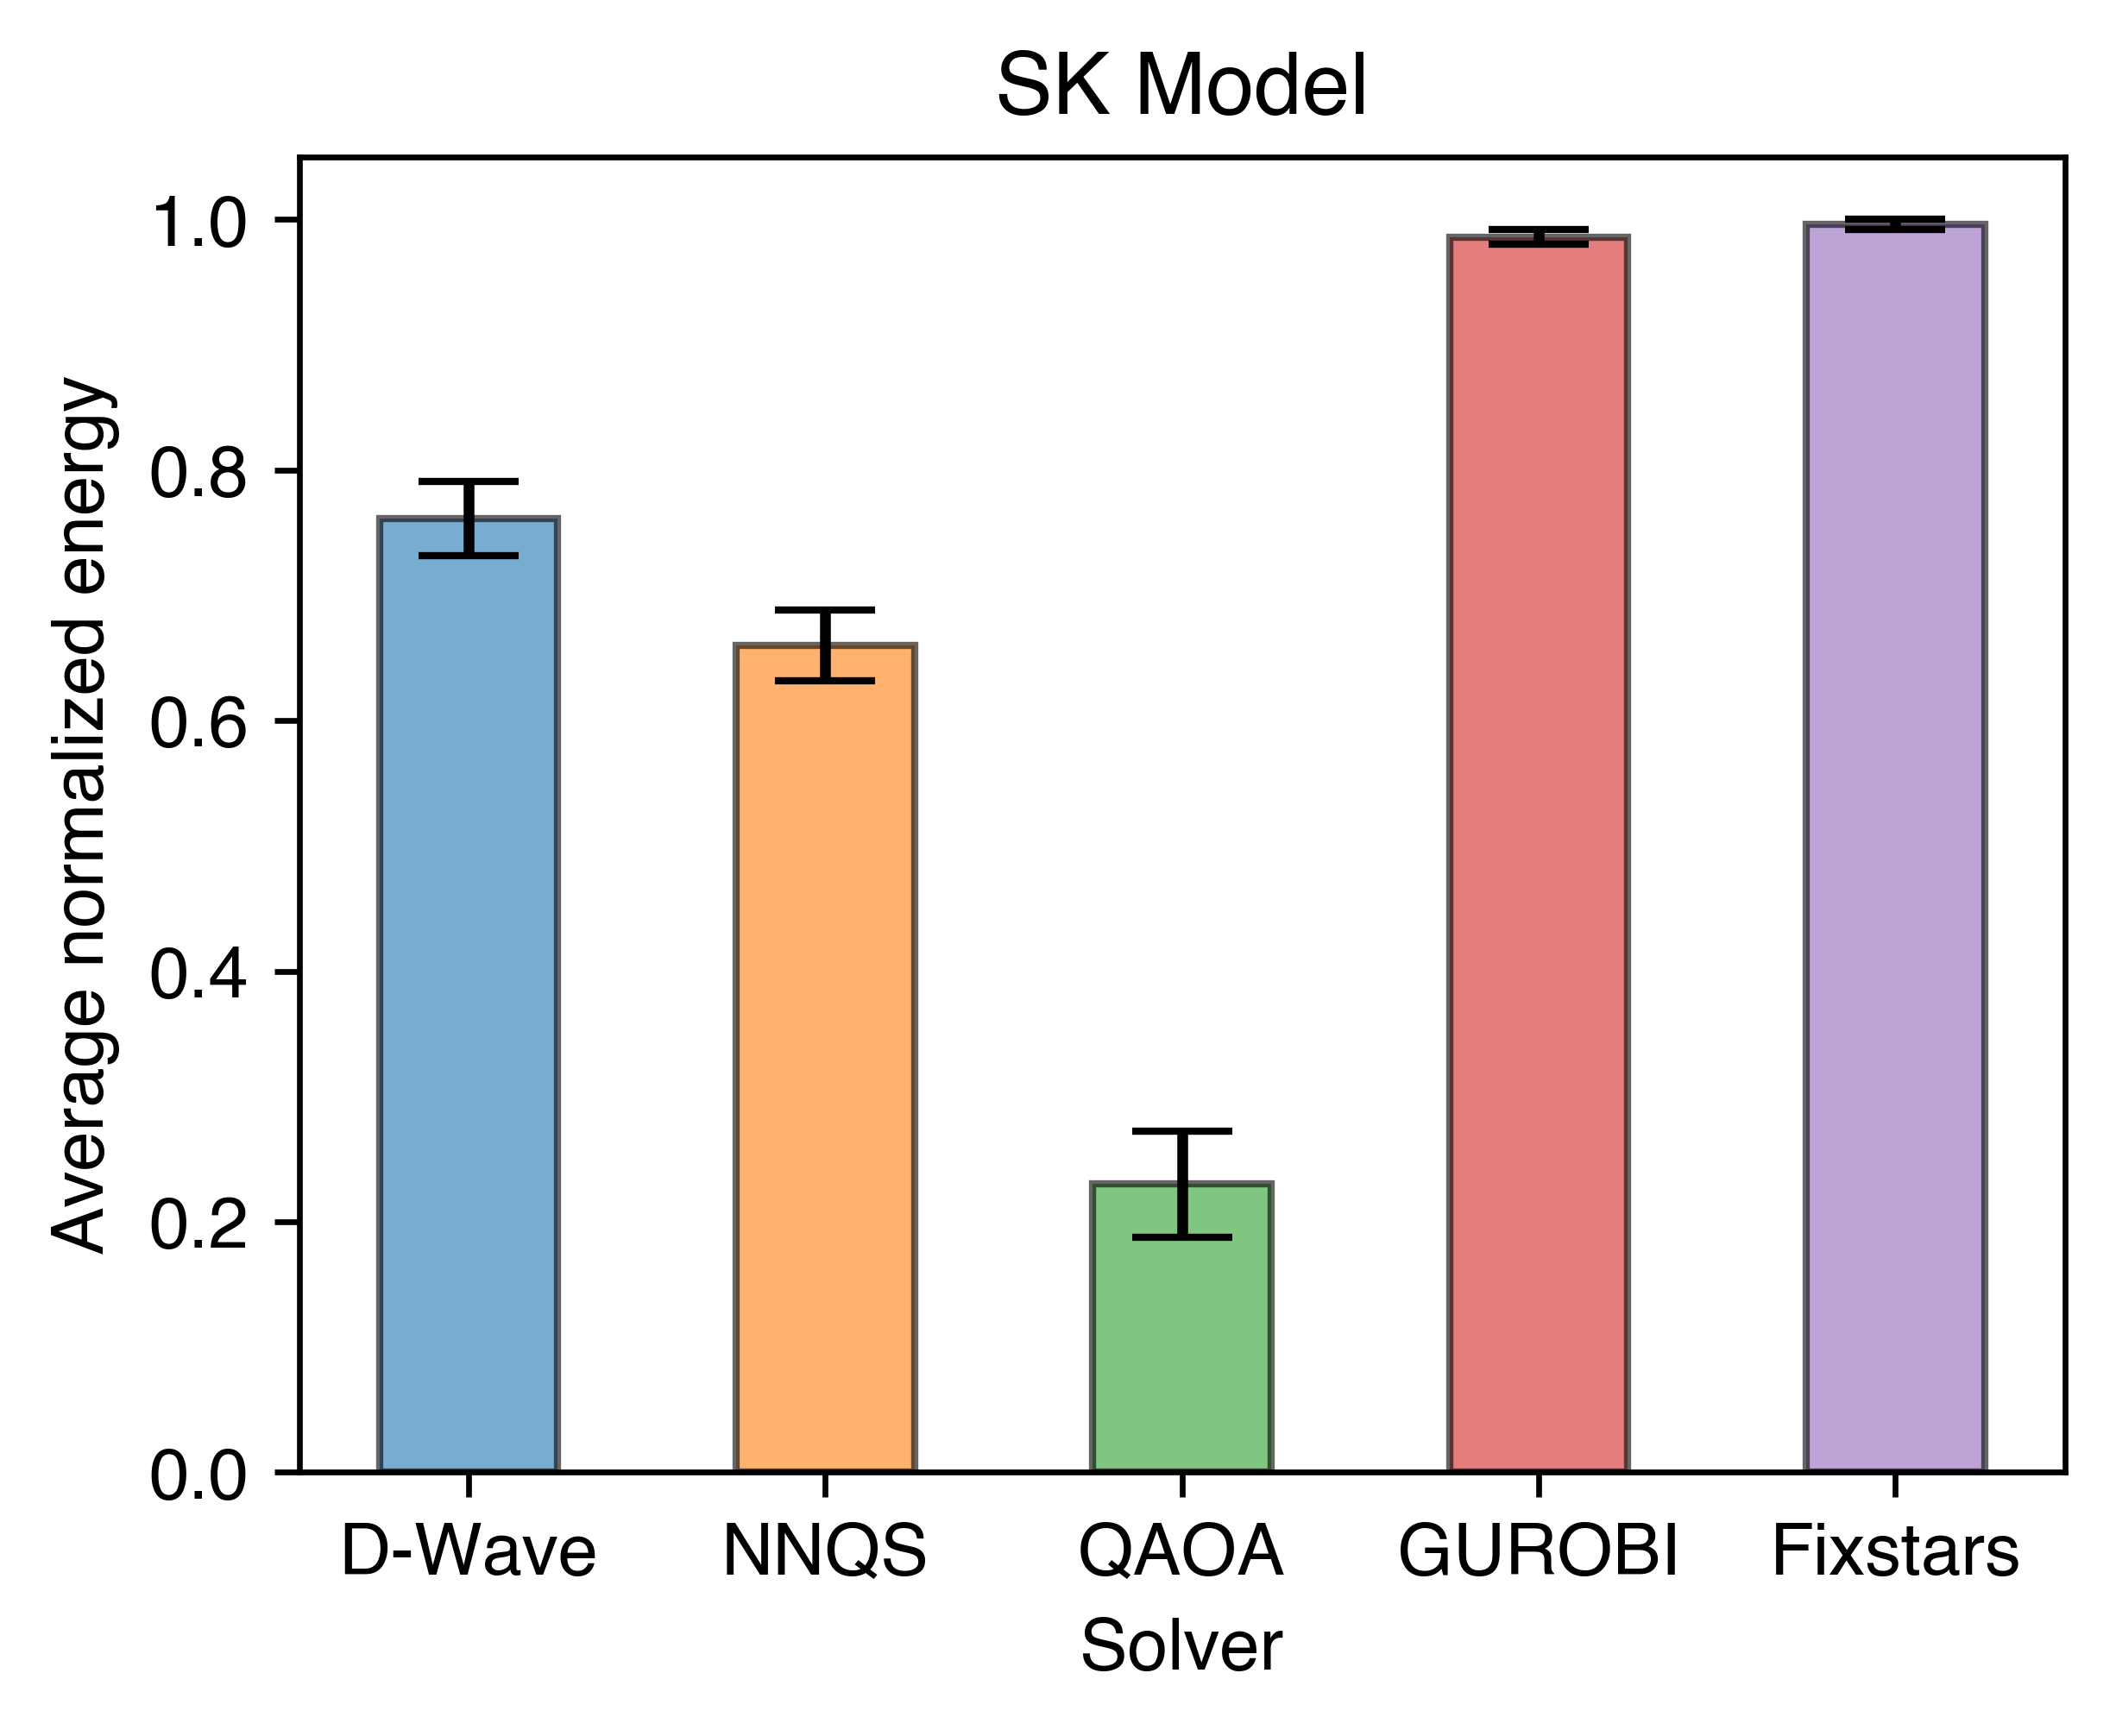
\includegraphics[width=0.49\textwidth]{images/skmodel_all_avg.png}}\hfill
    \subfloat[Success probability]{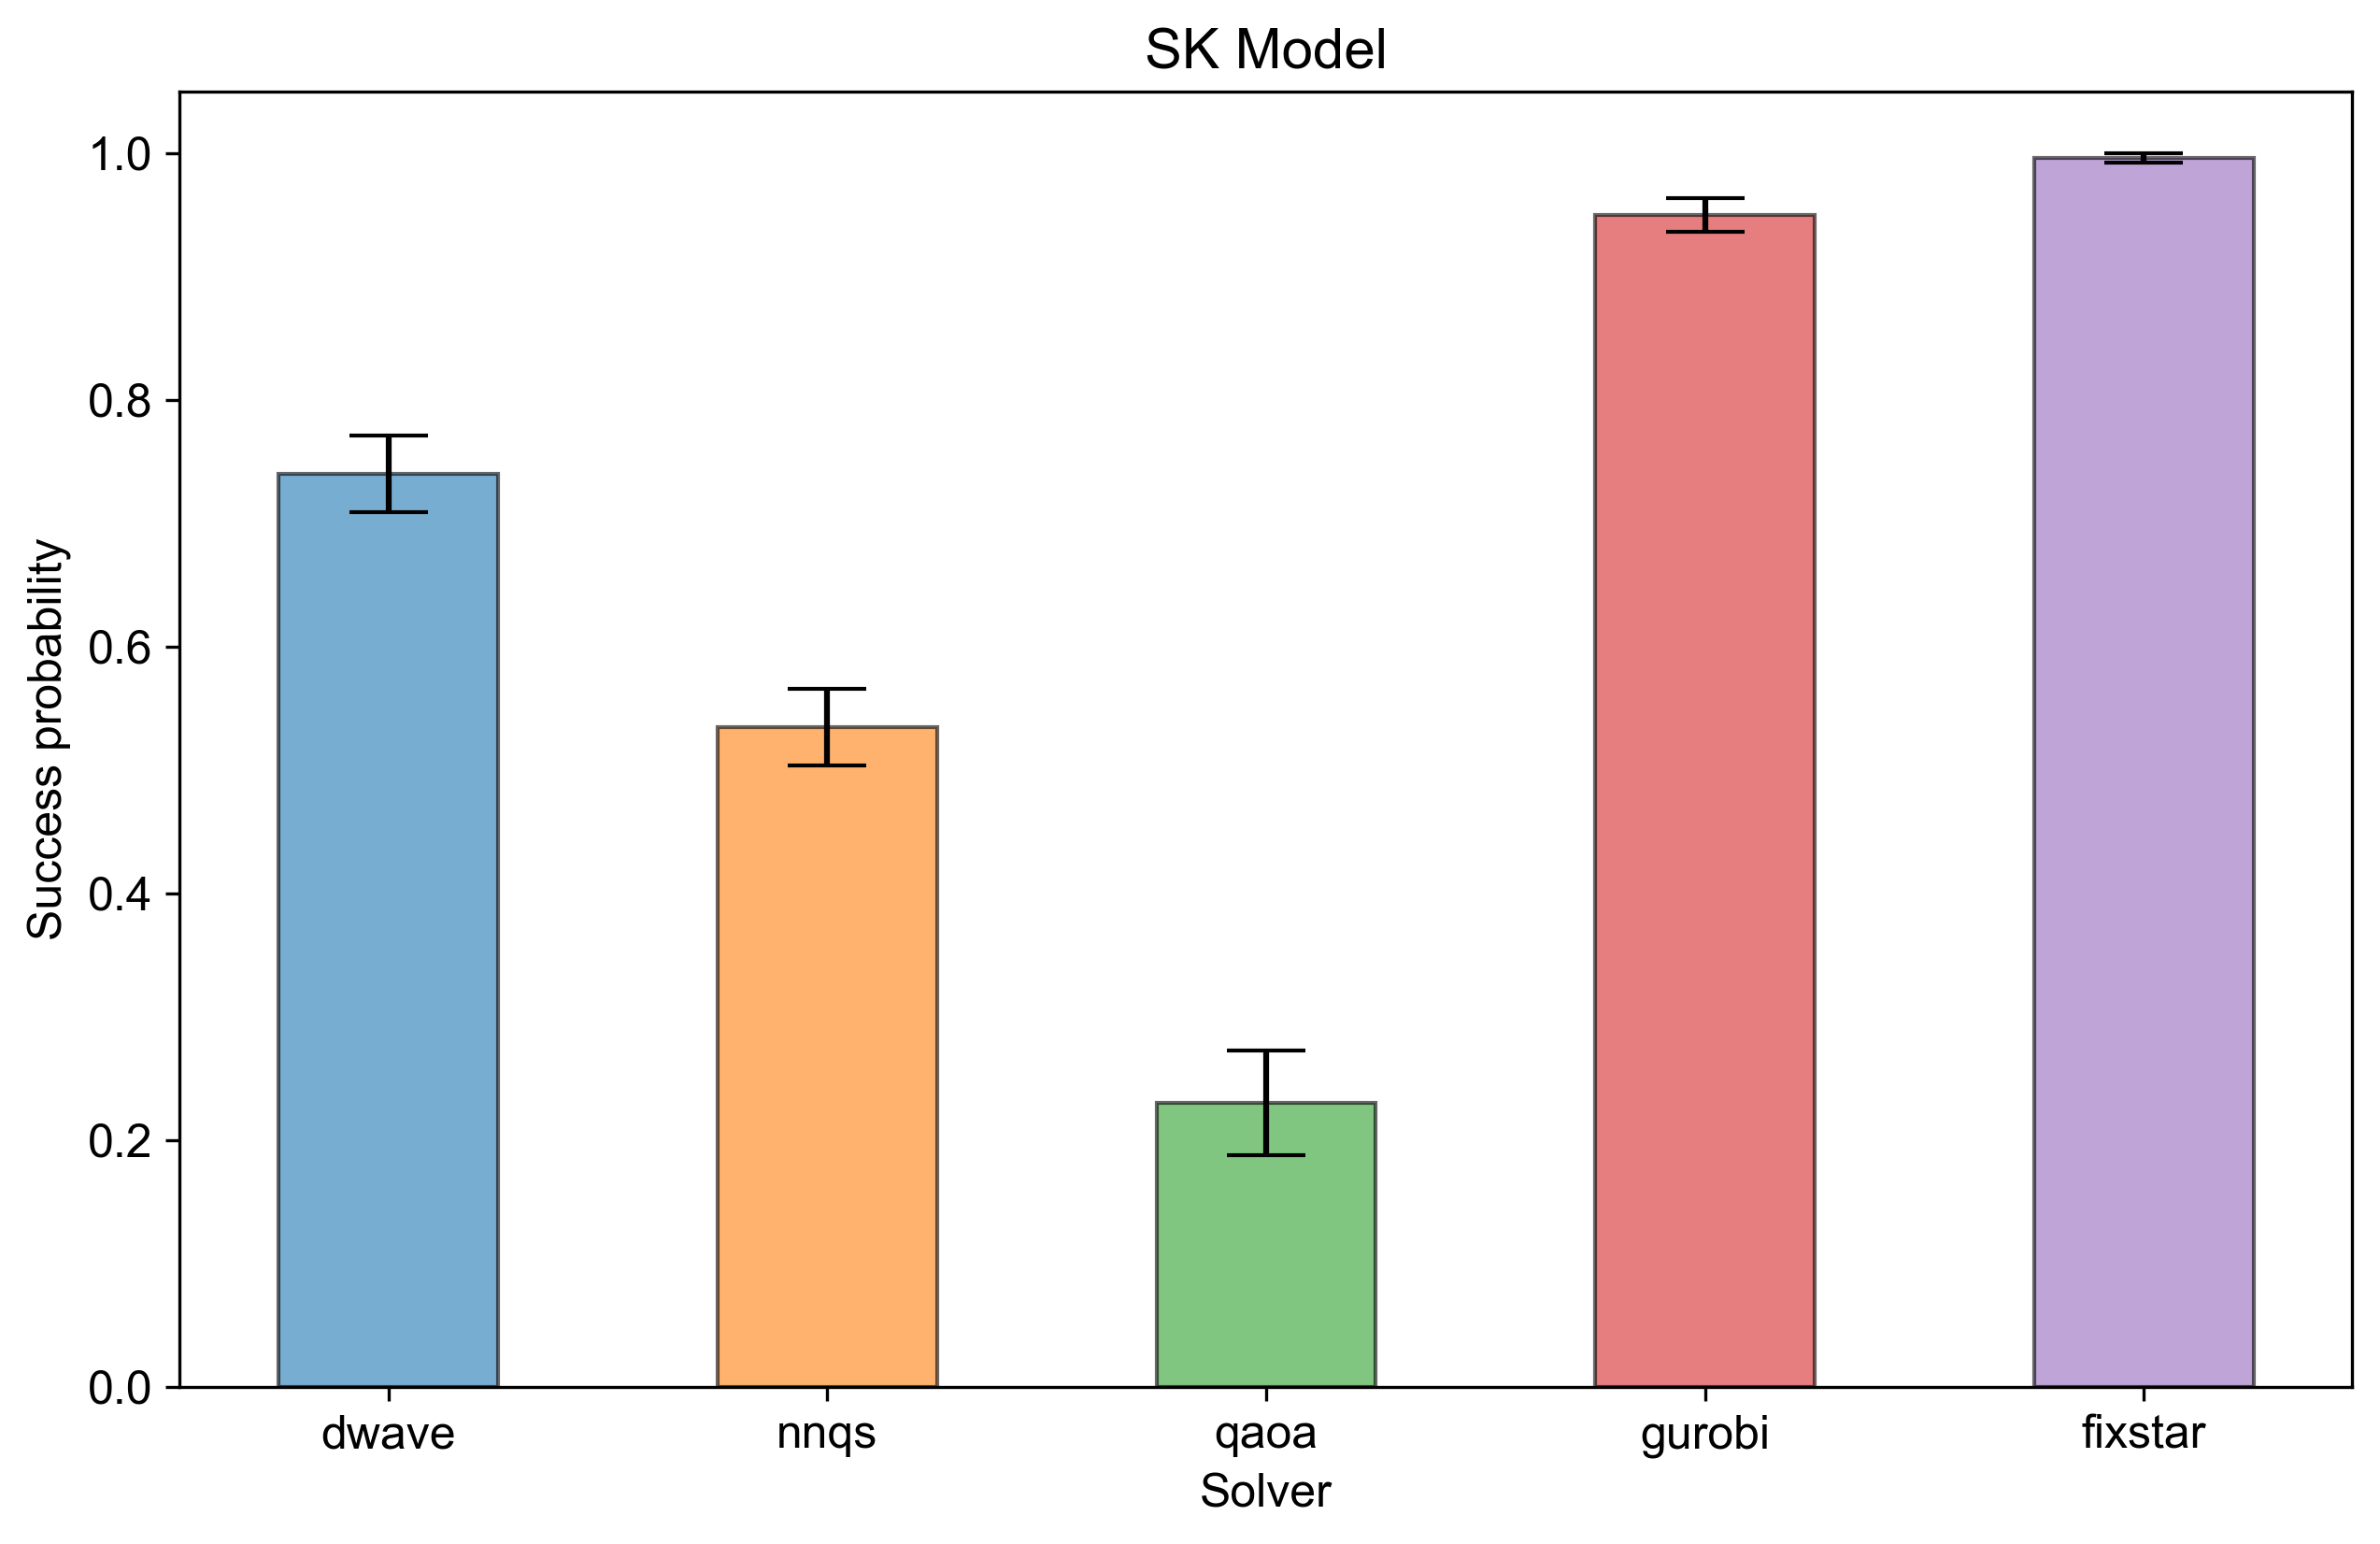
\includegraphics[width=0.49\textwidth]{images/skmodel_all_success_avg.png}}
    \caption{Average performance of different solvers for SK model}
    \label{all-skmodel-average}
\end{figure}

Performance by size for the SK model dataset is shown in \autoref{all-skmodel-size} and average performance is shown in \autoref{all-skmodel-average}. For the SK model, the D-wave solver could only handle problem sizes up to $n=150$ due to the need for minor embedding onto the pegasus topology. The SK model is fully connected which makes embedding difficult for the D-wave QPU. QAOA was able to solve problems of up to $n=30$ due to the limitations of the simulator.

The SK model presents a difficult problem for all QUBO solvers due to its multi-valley energy landscape and performance is much less consistent. The D-wave solver performs well up to $n=30$, with performance gradually decreasing for larger problems. The NNQS follows a similar trend, although it can solve problems of larger sizes and performs better at sizes of $=100,150$. The QAOA solver has consistently poor performance across problem sizes.

Overall, the D-wave annealer has the highest average normalized energy and success probability among the 3 quantum-inspired solvers. The NNQS is slightly worse in both metrics while the QAOA solver performs poorly in both metrics.

\section{Conclusion}
\autoref{results:allnormalizedenergy} and \autoref{results:allsuccess} show the average normalized energy and success probability for different solvers for each dataset and the average across all datasets.

When comparing the 3 quantum-inspired solvers, NNQS has the best normalized energy for the NAE3SAT and max-cut dataset while the D-wave solver has the best normalized energy for the SK model performance. NNQS also does the best in normalized energy when averaged across the 3 datasets. 

QAOA has the best success probability for the NAE3SAT dataset. However, it is important to note that it was only able to handle problems with up to $30$ variables. The D-wave solver has the best success probability for the max-cut and SK model datasets and the success probability averaged across the 3 datasets.

\begin{table}[!ht]
    \centering
    \begin{tabular}{cccccc} \toprule
        ~ & D-wave & NNQS & QAOA & GUROBI & Fixstar \\ \midrule
        NAE3SAT & 0.617 & \textbf{0.755} & 0.640 & 0.983 & 1.00 \\
        Max-cut & 0.610 & \textbf{0.783} & 0.190 & 0.983 & 1.00 \\
        SK model & \textbf{0.691} & 0.646 & 0.178 & 0.870 & 0.910 \\ \midrule
        Average & 0.640 & \textbf{0.728} & 0.336 & 0.946 & 0.970 \\ \bottomrule
    \end{tabular}
    \caption{Average normalized energy for different solvers}
    \label{results:allnormalizedenergy}
\end{table}

\begin{table}[!ht]
    \centering
    \begin{tabular}{cccccc} \toprule
        ~ & D-wave & NNQS & QAOA & GUROBI & Fixstar \\ \midrule
        NAE3SAT & 0.617 & \textbf{0.755} & 0.640 & 0.983 & 1.00 \\
        Max-cut & 0.610 & \textbf{0.783} & 0.190 & 0.983 & 1.00 \\
        SK model & \textbf{0.691} & 0.646 & 0.178 & 0.870 & 0.910 \\ \midrule
        Average & 0.640 & \textbf{0.728} & 0.336 & 0.946 & 0.970 \\ \bottomrule
    \end{tabular}
\caption{Success probability for different solvers}
\label{results:allsuccess}
\end{table}

